\documentclass[a4paper]{article}

%% Language and font encodings
\usepackage[english]{babel}
\usepackage[utf8x]{inputenc}
\usepackage[T1]{fontenc}
\usepackage{amsmath}
\usepackage{mlka_math}

%% Sets page size and margins
\usepackage[a4paper,top=3cm,bottom=2cm,left=3cm,right=3cm,marginparwidth=1.75cm]{geometry}

%% Useful packages
\usepackage{amsmath}
\usepackage{amsthm}
\usepackage{amssymb}
\usepackage{graphicx}
\usepackage[colorinlistoftodos]{todonotes}
\usepackage[colorlinks=true, allcolors=blue]{hyperref}
\usepackage{neuralnetwork}
\usepackage{sidecap}

\newtheorem{theorem}{Theorem}[section]
\newtheorem{corollary}{Corollary}[theorem]
\newtheorem{lemma}[theorem]{Lemma}



\title{Cheatsheet for Fisher-Rao Metric, Geometry, and Complexity of Neural Networks}
\author{Sandro Braun, Leander Kurscheidt}


%%% --- commands ---

%network notation with nonlinearities
\def\basicNN{
	{
		\sigma_{L+1}(
		\sigma_{L}(
		\cdots 
		\sigma_{2}(
		\sigma_1(
		x^T W^0)
		W^1)
		W^2)
		\cdots)
		W^L)
	}
}

\def\structuredNN{
	{
		x^T W^0 D^1(x) W^1 D^2(x) \dots D^L W^L D^{L+1}(x)
	}
}






\begin{document}
\maketitle
\begin{abstract}
\end{abstract}
\section{Geometry of Deep Rectified Networks}


\subsection{Lemma 2.1}

\begin{lemma}[Structure in Gradients]
	\begin{align}
		\label{lemma_structure_in_gradient}
		\sum_{t=0}^{L} \sum_{i \in [k_t], j \in [k_{t+1}]} \frac{\partial O^{L+1}}{\partial W^{t_{ij}}} W^t_{ij} = (L+1)O^{L+1}(x) = \langle \nabla_\theta f_\theta (x), \theta \rangle
	\end{align}
\end{lemma}

\subsubsection{Example for Lemma 2.1 with single output}

Take a simple feed forward neural network with only two inputs and one output. Remember that by definition $O^0 = x$.
Illustrated: \\

\begin{neuralnetwork}[height=2]
	\newcommand{\nodetextx}[2]{$x_#2$}
	\newcommand{\nodetexty}[2]{$y_#2$}
	\inputlayer[count=2, bias=false, title=$O^0$, text=\nodetextx]
	\outputlayer[count=1, title=$O^1$, text=\nodetexty] \linklayers
\end{neuralnetwork}

The simple example can then be written with:

\begin{align}
	\label{eq_simple_nn}
	O^0 = 	\begin{bmatrix}
				O^0_1 \\ 
				O^0_2
			\end{bmatrix} &,
	W^0 = 	\begin{bmatrix}
				W^0_1 \\
				W^0_2
			\end{bmatrix} \\
			O^1 &= \sigma({O^0}^T W^0) = \sigma(
											\underbrace{O^0_1 W^0_1 + O^0_2 W^0_2}_z
											).
\end{align}
Substituting the term in brackets will simplify notation.

%\begin{minipage}{.5\textwidth}
Now calculate the partial derivatives of \eqref{eq_simple_nn} with respect to $W^0_i$.
\begin{align*}
	\frac{\partial O^1}{\partial W^0_1} &= \sigma'(z) O^0_1 \\
	\frac{\partial O^1}{\partial W^0_2} &= \sigma'(z) O^0_2
\end{align*}
Summing up the $\frac{\partial O^1}{\partial W_j} W_j$ reveals,

\begin{align*}
	\sum_{j=1}^{2} \frac{\partial O^1}{\partial W^0_j} W^0_j &= \sigma'(z) O^0_1  W^0_1 + \sigma'(z) O^0_2  W^0_2 = \sigma'(z)(\underbrace{O^0_1 W^0_1 + O^0_2 W^0_2}_\text{z}) \\
														&= \sigma'(z) z
\end{align*}
Note that this is equivalent to calculating $\langle \nabla_{W^0} O^1, W^0 \rangle$:
\begin{align*}
	\nabla_{W^0} O^1 &= 
		\begin{bmatrix}
			\frac{\partial O^1}{\partial W^0_1} \\ 
			\frac{\partial O^1}{\partial W^0_2}
		\end{bmatrix} \\
	\langle \nabla_{W^0} O^1, W^0 \rangle &= \sum_{j=1}^{2} \frac{\partial O^1}{\partial W^0_j} W^0_j = \dots = \sigma'(z) z
\end{align*}
Using the relation $\sigma(z) = \sigma'(z)(z)$ reveals \eqref{eq_simple_nn}. Then reading left to right reveals \eqref{lemma_structure_in_gradient} for $L=0$, $\theta= W^0$ and $f_\theta(x) = O^1(x)$ which completes the example.

\begin{align*}
		\sum_{t=0}^{L=0} \sum_{j=1}^{2} \frac{\partial O^1}{\partial W^t_j} W^t_j
		=  \langle \nabla_{W^0} O^1, W^0 \rangle
		= \sigma'(z) z 
		= \sigma(z) = O^1
\end{align*}

%\end{minipage}%

\subsubsection{Applying Lemma 2.1 to the network structure}

Lemma 2.1 applied to the network notation leads to the following notation:

\begin{align}
	\label{eq:lemma2_1}
	\text{Lemma 2.1} : \sigma(z) &= \sigma'(z) z \\
	\label{eq:basicNN}
	\text{Network notation} : f_\theta(x) &= \basicNN \\
	\label{eq:structuredNN}
	\text{combined} : f_\theta(x) &= \structuredNN
\end{align}

\subsubsection{Example for Lemma 2.1 with multiple outputs}
	Take again a simple neural network consisting of a single layer, hence $L=0$. We will now start from \eqref{eq:basicNN} for $L=0$, then use \eqref{eq:lemma2_1} to get \eqref{eq:structuredNN}.
	Now assume, w.l.o.g. the network has two inputs and two outputs. We then have
	\begin{align}
	O^0 &= 	\begin{bmatrix}
				O^0_1 \\ 
				O^0_2
			\end{bmatrix}, ~
	O^1 = 	\begin{bmatrix}
				O^1_1 \\ 
				O^1_2
			\end{bmatrix}, ~
	W^0 = 	\begin{bmatrix}
				W^0_{1,1}  & W^0_{1,2} \\ 
				W^0_{2,1}  & W^0_{2,2}
			\end{bmatrix},	\\
	\label{eq:2_output_example}
	O^1 &=
			\sigma(O^{0^T} W^0) \\
		&=
			\sigma(
			\begin{bmatrix}
				O^0_1 W^0_{1,1}  + O^0_2 W^0_{1,2} \\
				O^0_1 W^0_{2,1}  + O^0_2 W^0_{2,2}
			\end{bmatrix})  \\
		&= 
			\begin{bmatrix}
				\sigma(O^0_1 W^0_{1,1}  + O^0_2 W^0_{1,2}) \\
				\sigma(O^0_1 W^0_{2,1}  + O^0_2 W^0_{2,2})
			\end{bmatrix} \\
		&= 
			\begin{bmatrix}
				\sigma(N^1_1) \\
				\sigma(N^1_2)
			\end{bmatrix} \\
	\end{align}
	For simplicity, we can replace the sum within each vector element with $N^1_i$. Now remember \eqref{eq:lemma2_1} and apply it to \eqref{eq:2_output_example}.
	\begin{align}
	O^1 &= 
			\begin{bmatrix}
				\sigma(N^1_1) \\
				\sigma(N^1_2)
			\end{bmatrix} \\
		&= 
			\begin{bmatrix}
				\sigma'(N^1_1) N^1_1 \\
				\sigma'(N^1_2) N^1_2
			\end{bmatrix} \\
		&=  
			\begin{bmatrix}
				N^1_1 & N^1_2
			\end{bmatrix}	
			\underbrace{
				\begin{bmatrix}
					\sigma'(N^1_1)	&	0\\
					0				&	\sigma'(N^1_2)
				\end{bmatrix}
			}_{D^1(x)} \\
		&=
			N^1 D^1(x)		
	\end{align}
	The last step is to remember $N^{i+1} = O^{i^\TT}W^1$, then we have
	\begin{align}
		O^1 &= 
				{O^0}^\TT W^0 D^1(x) \\
			&= 
				{x}^\TT W^0 D^1(x)
	\end{align}
	which is equivalent to inserting $L=0$ to \eqref{eq:structuredNN}. This completes the example.
	

\subsection{Corollary 2.1}

\subsubsection{Notes}
\begin{enumerate}
	\item 
	\begin{proof}
		We want to show $\frac{\partial l(f,Y)}{\partial f} = -y \Leftrightarrow yf < 1$. So,
		\begin{alignat*}{2}
			                && 1-y_if_i &> 0 \\
			\Leftrightarrow && l &=1-y_if_i \\
			\Leftrightarrow && \frac{\partial l}{\partial f} &=-y_i
		\end{alignat*}
	  \end{proof}
	\item 
	\begin{proof}
		We want to show $\frac{\partial l(f,Y)}{\partial f} = 0 \Leftrightarrow yf > 1$. So,
		\begin{alignat*}{2}
							&& 1-y_if_i &< 0 \\
			\Leftrightarrow && l &=0 \\
			\Leftrightarrow && \frac{\partial l}{\partial f} &=0
		\end{alignat*}
	  \end{proof}
\end{enumerate}


\begin{figure}[htb]
	\centering
	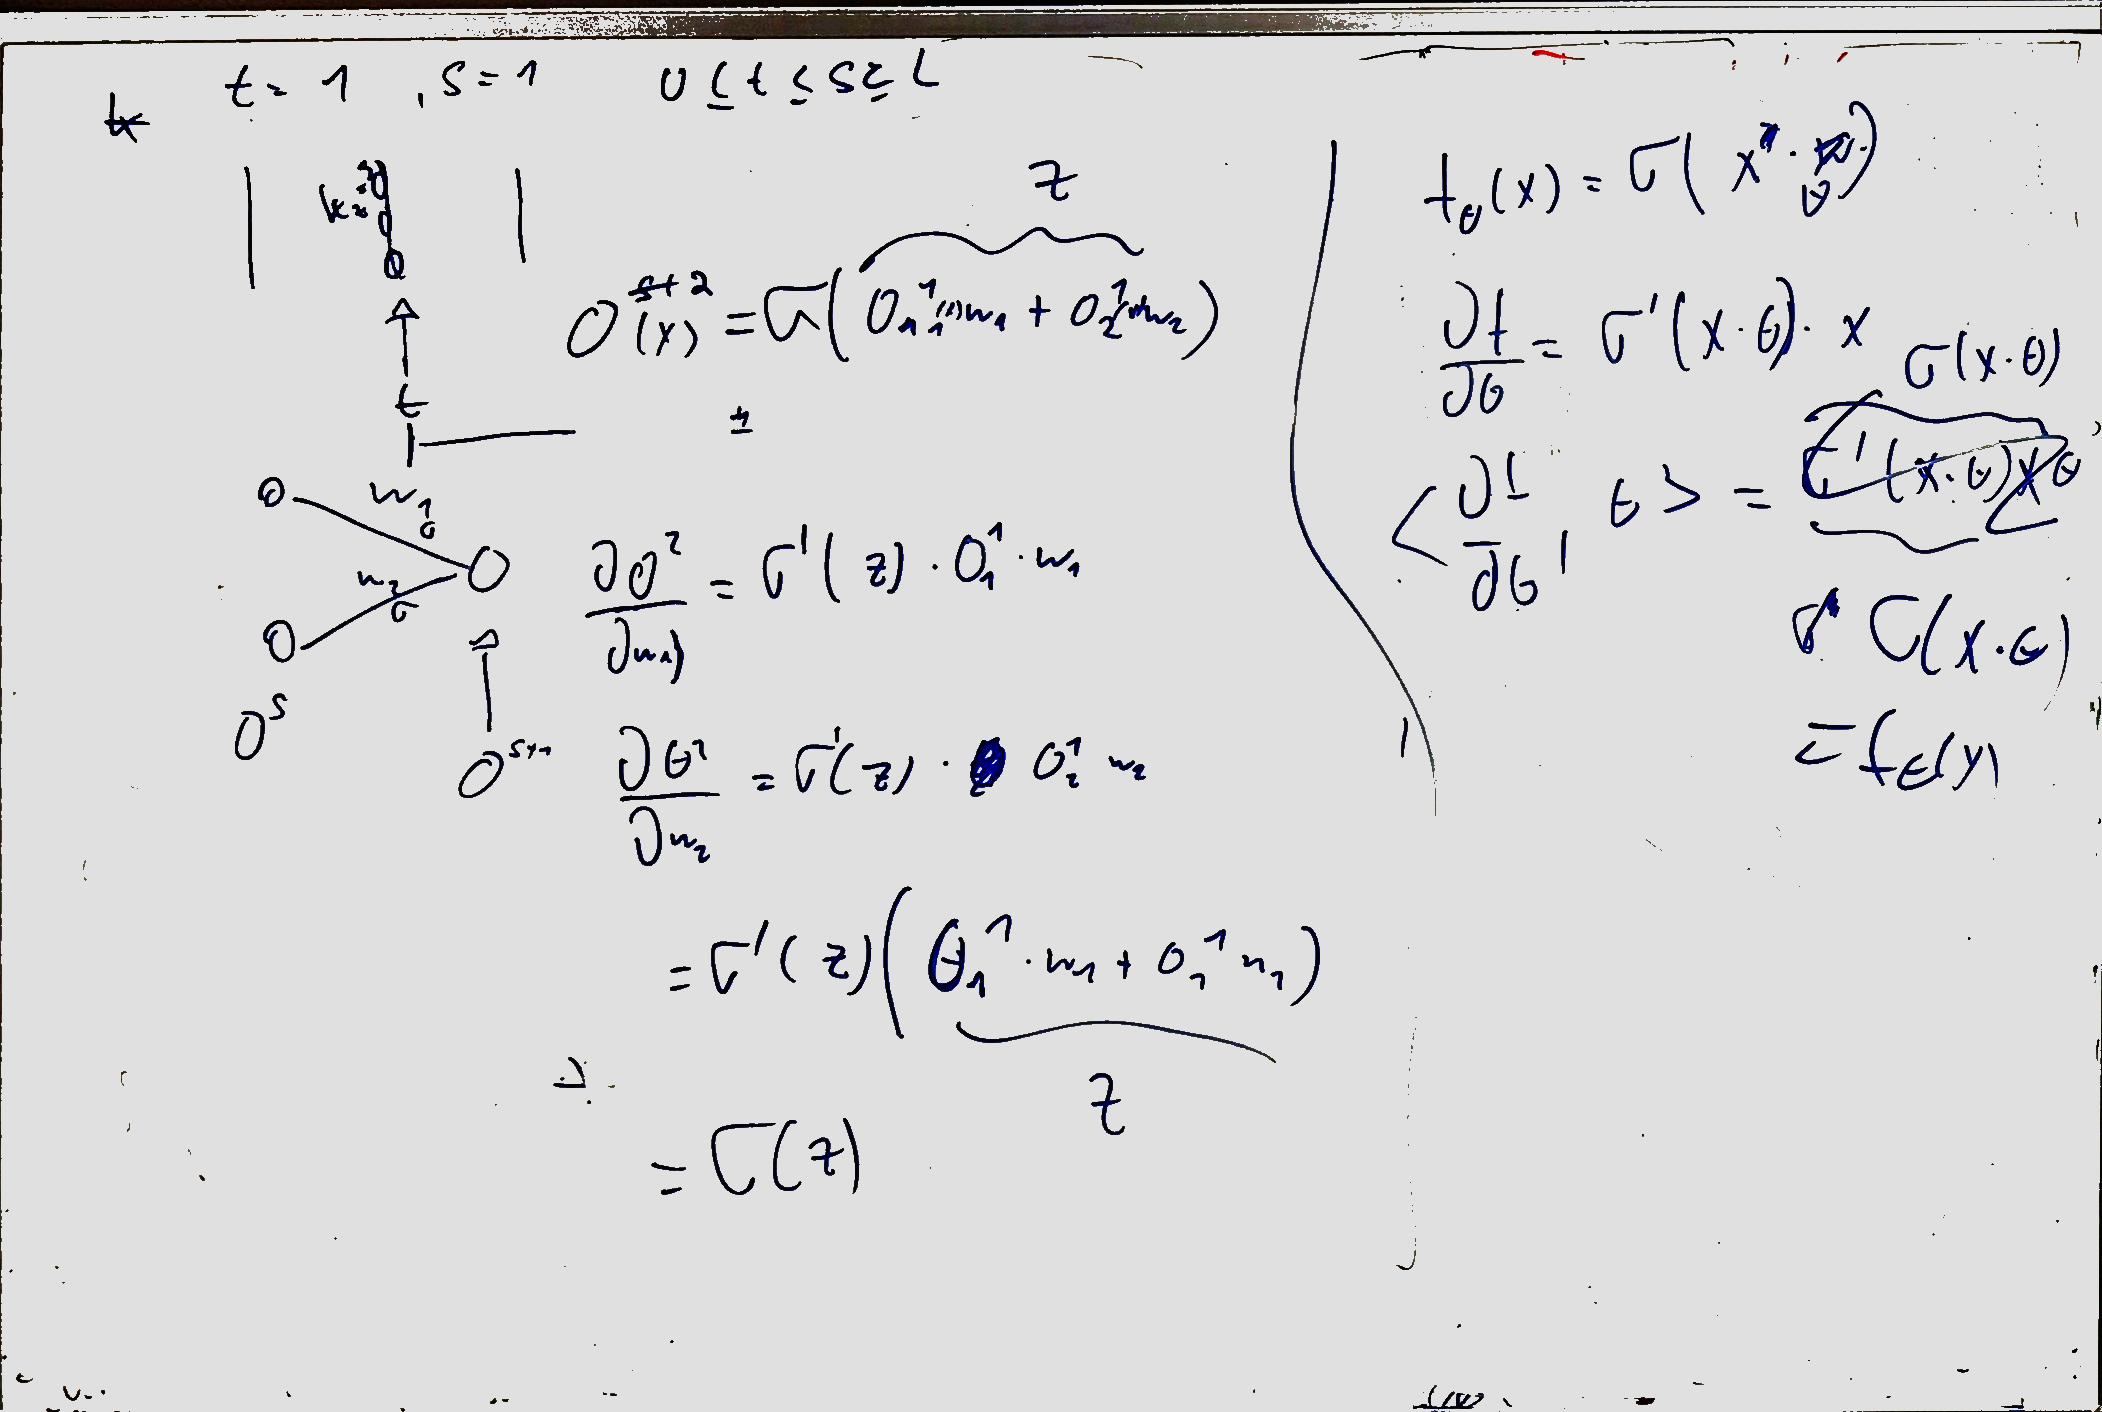
\includegraphics[width=\textwidth]{whiteboard_notes/01.jpg}
\end{figure}

\begin{figure}[htb]
	\centering
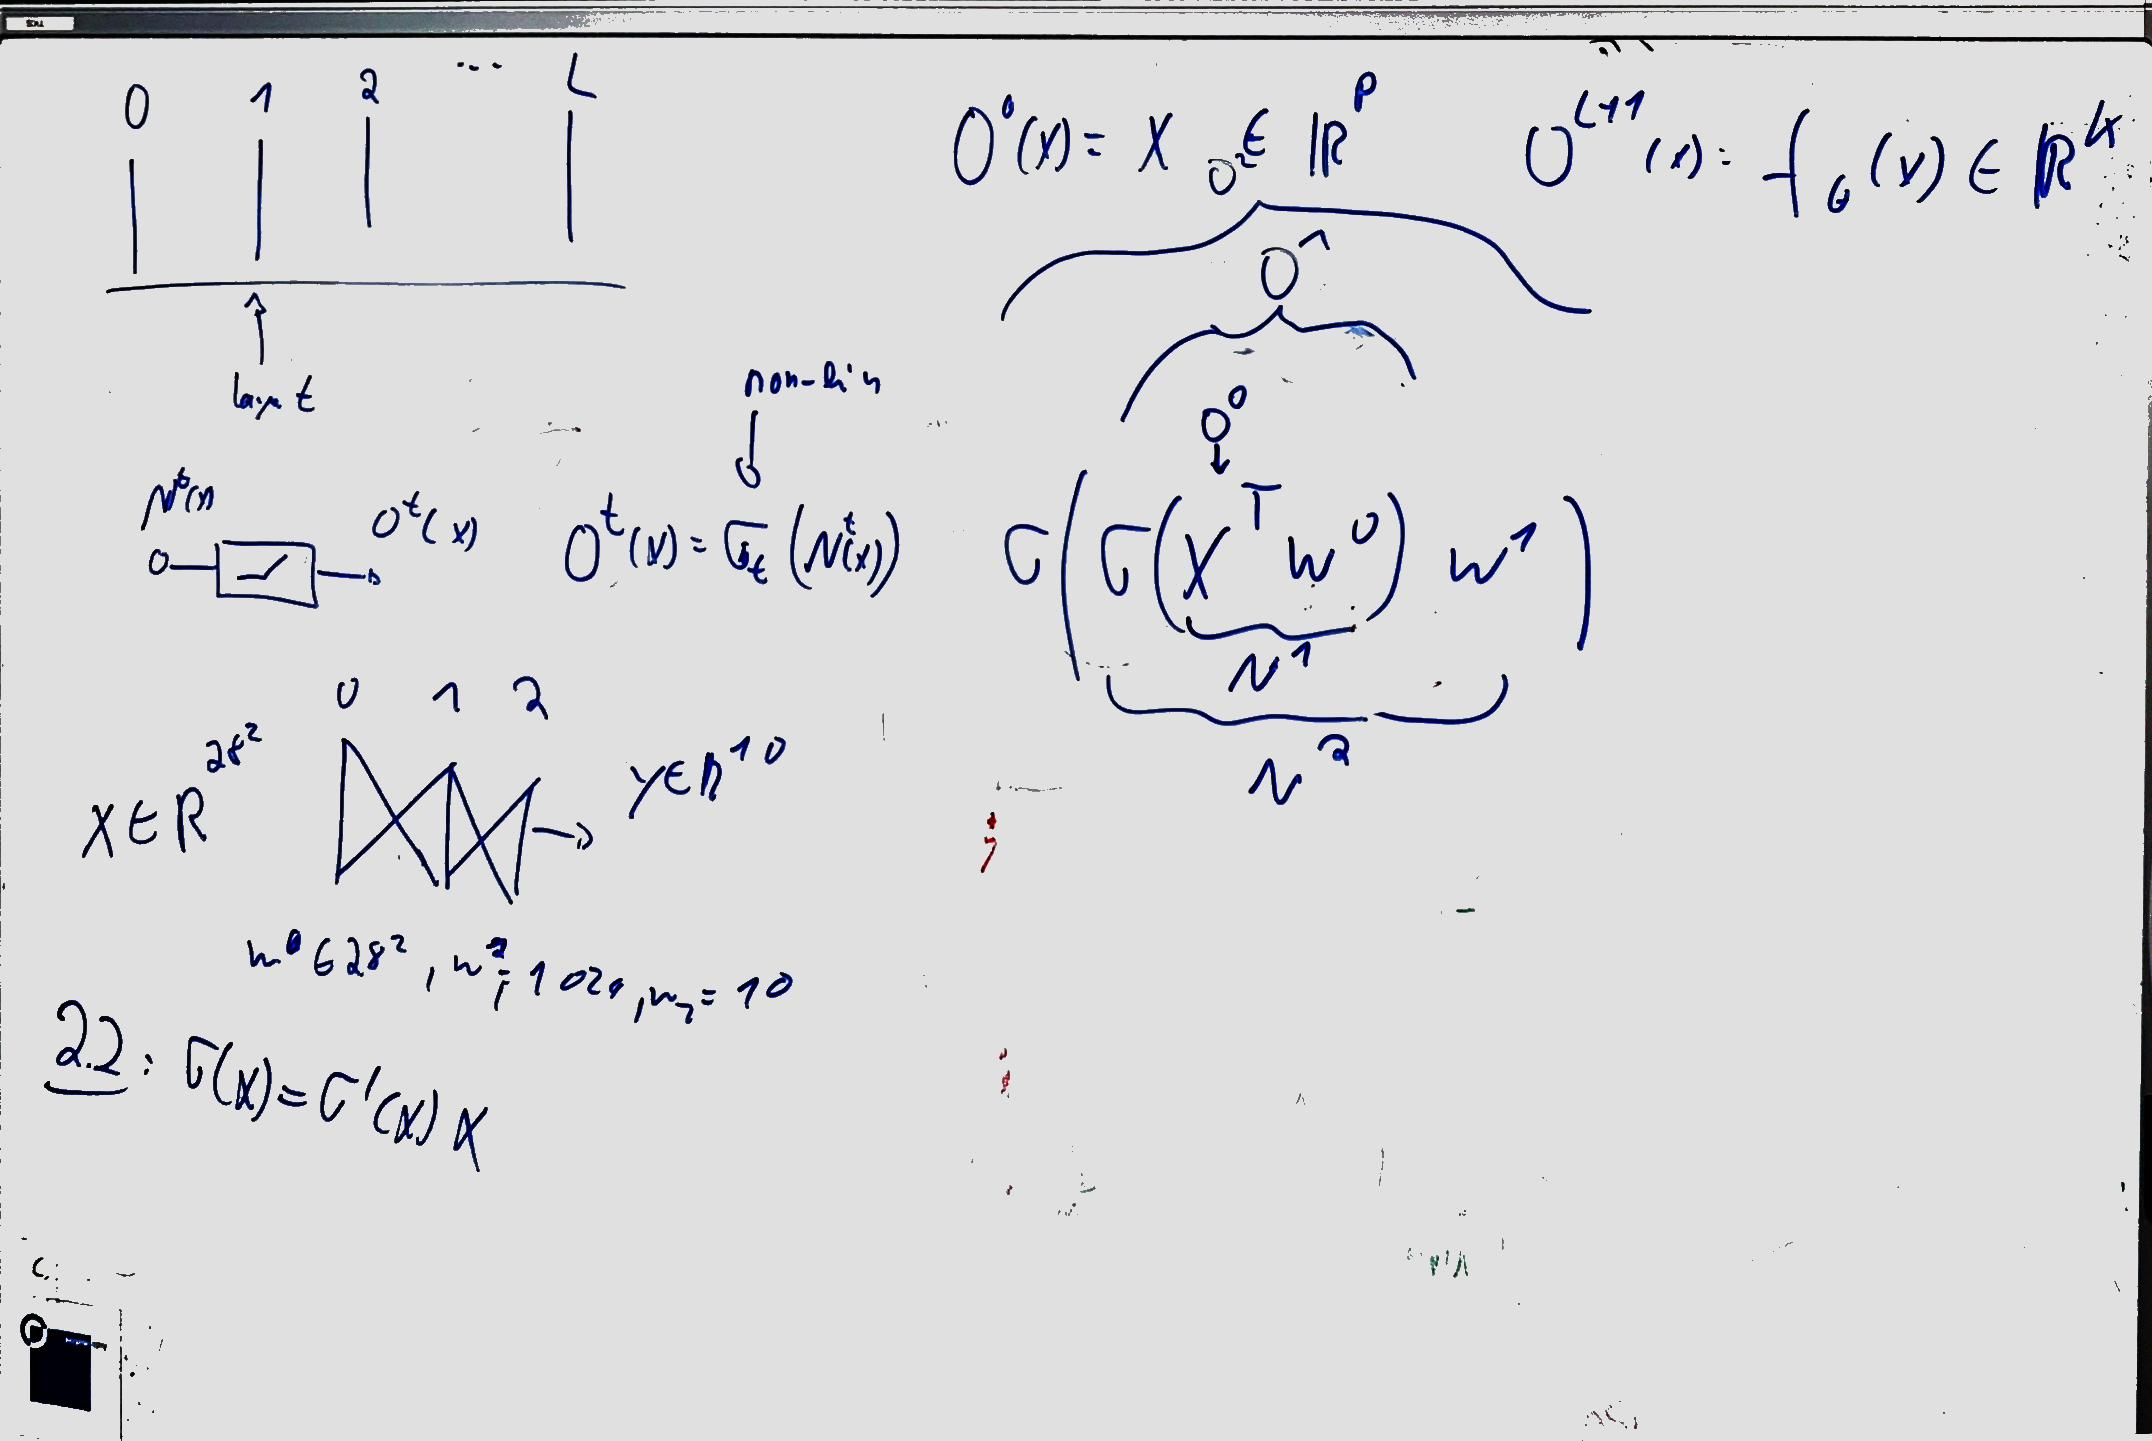
\includegraphics[width=\textwidth]{whiteboard_notes/02.jpg}
\end{figure}
\begin{figure}[htb]
	\centering
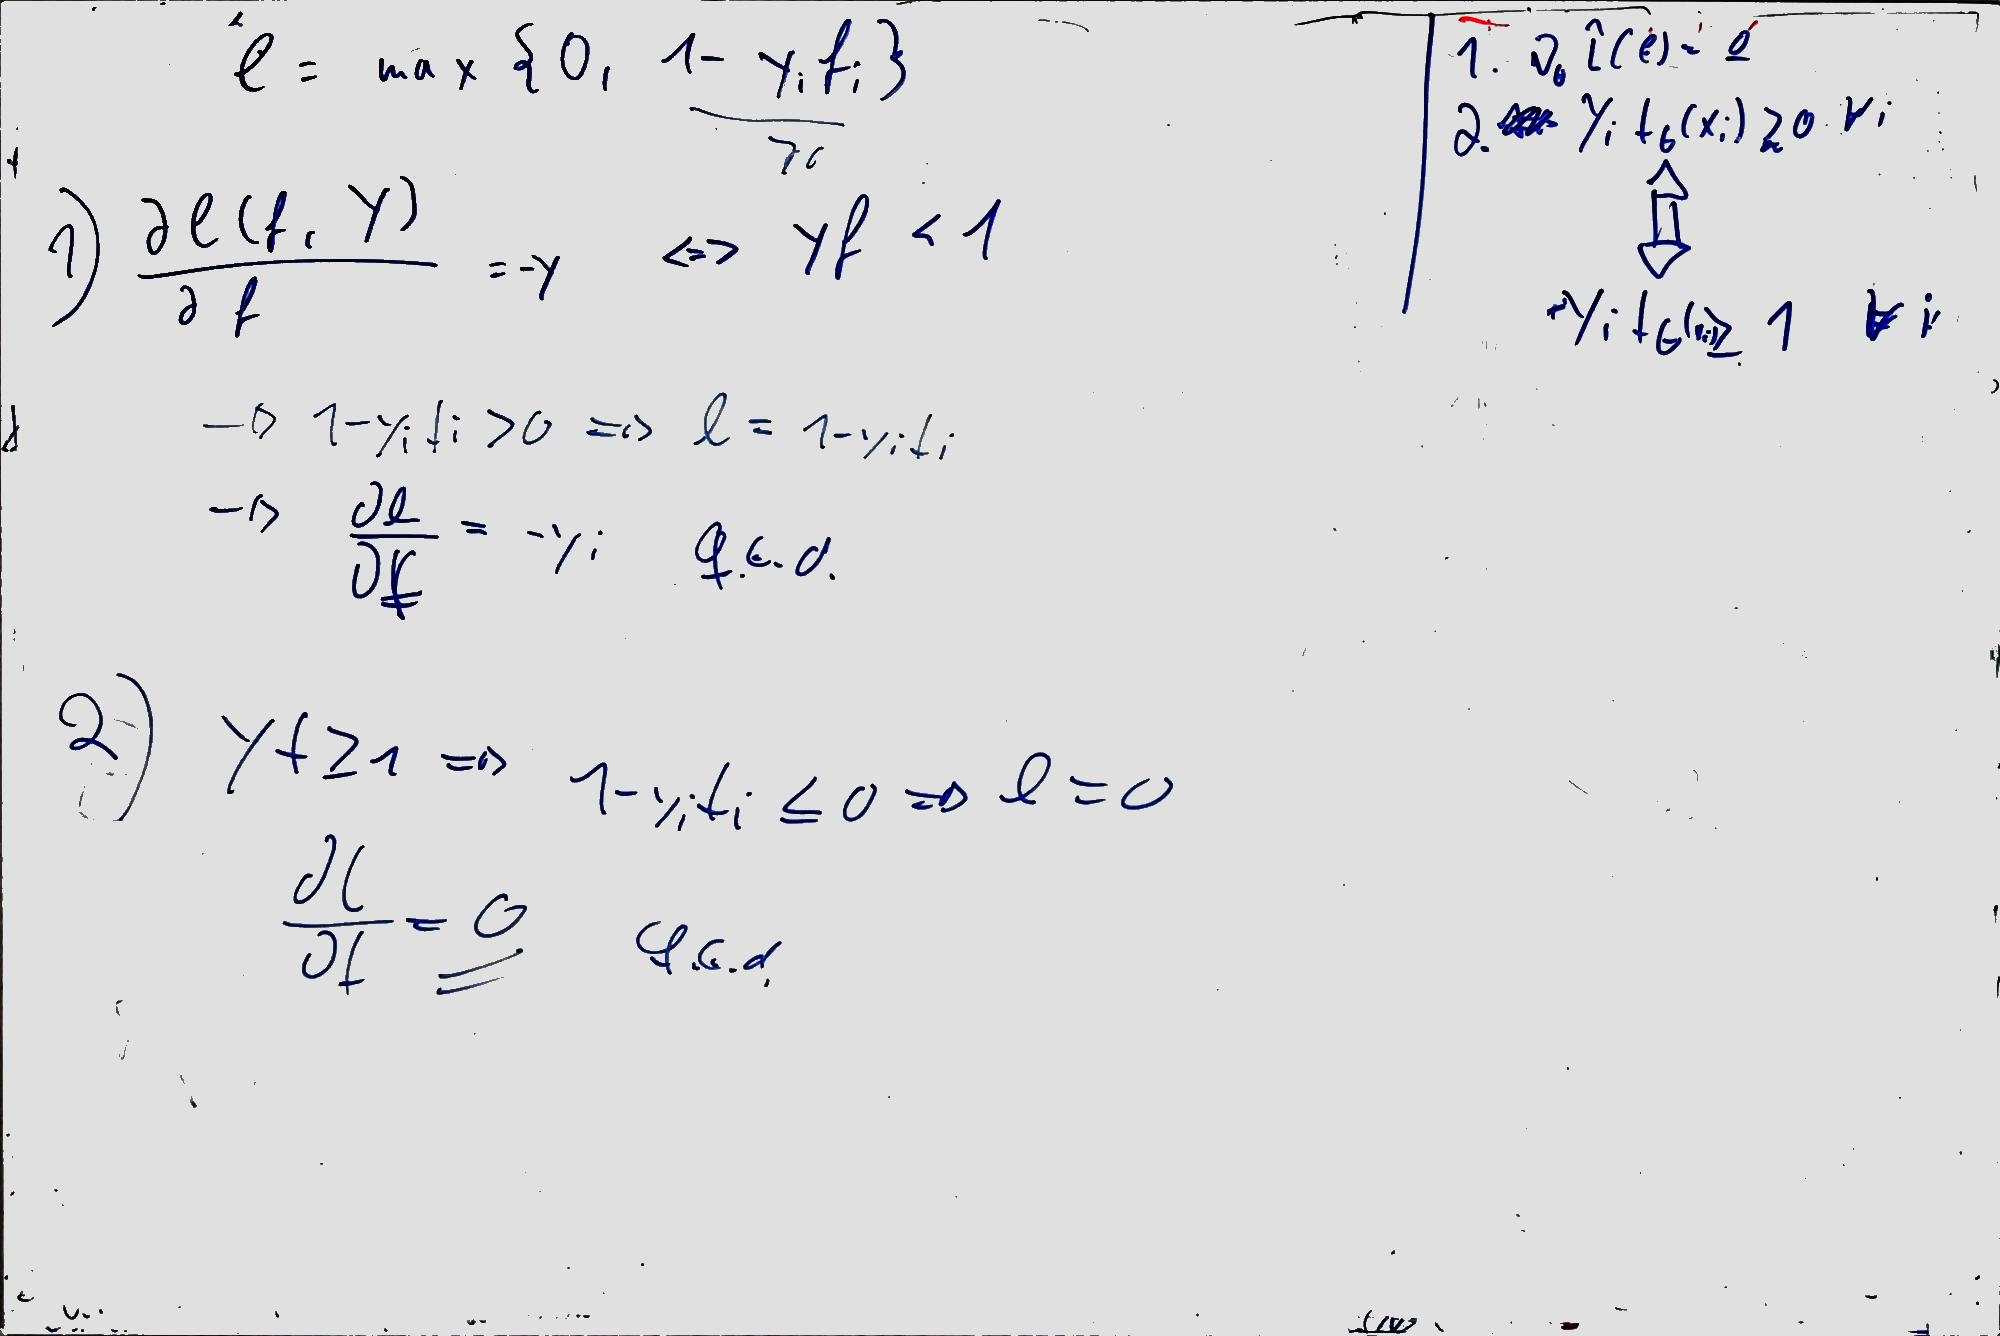
\includegraphics[width=\textwidth]{whiteboard_notes/03.jpg}
\end{figure}
\begin{figure}[htb]
	\centering
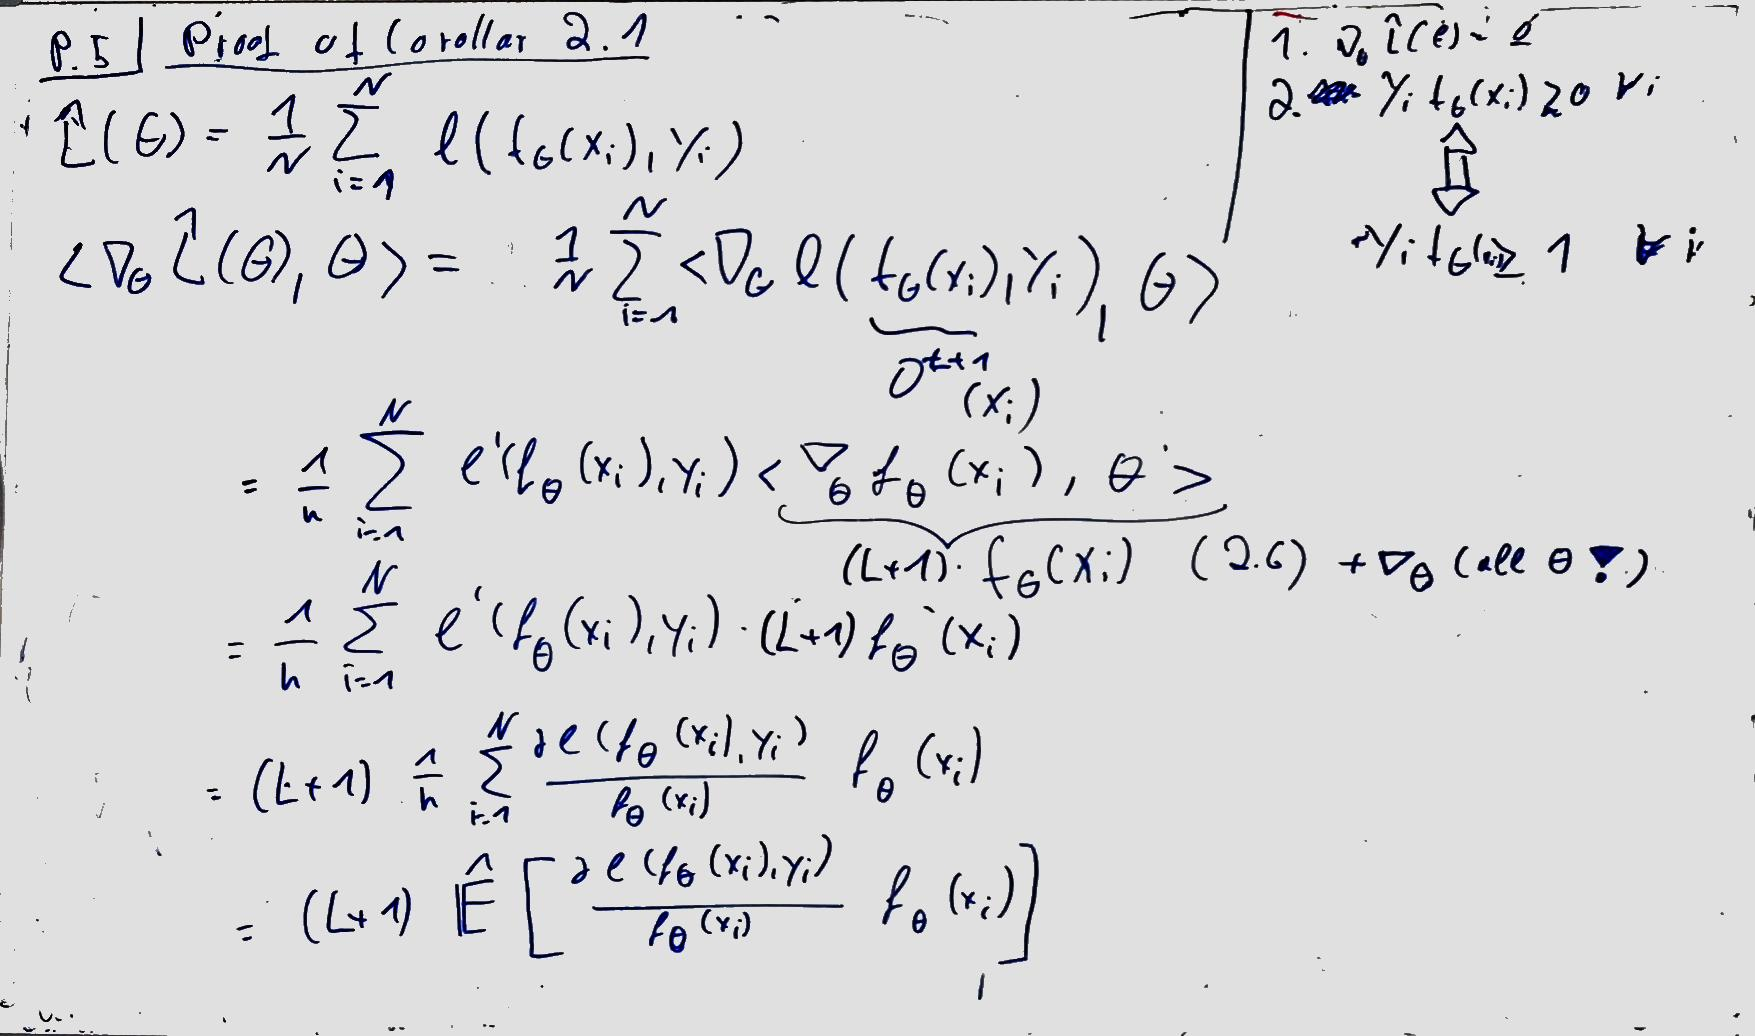
\includegraphics[width=\textwidth]{whiteboard_notes/04.jpg}
\end{figure}
\begin{figure}[htb]
	\centering
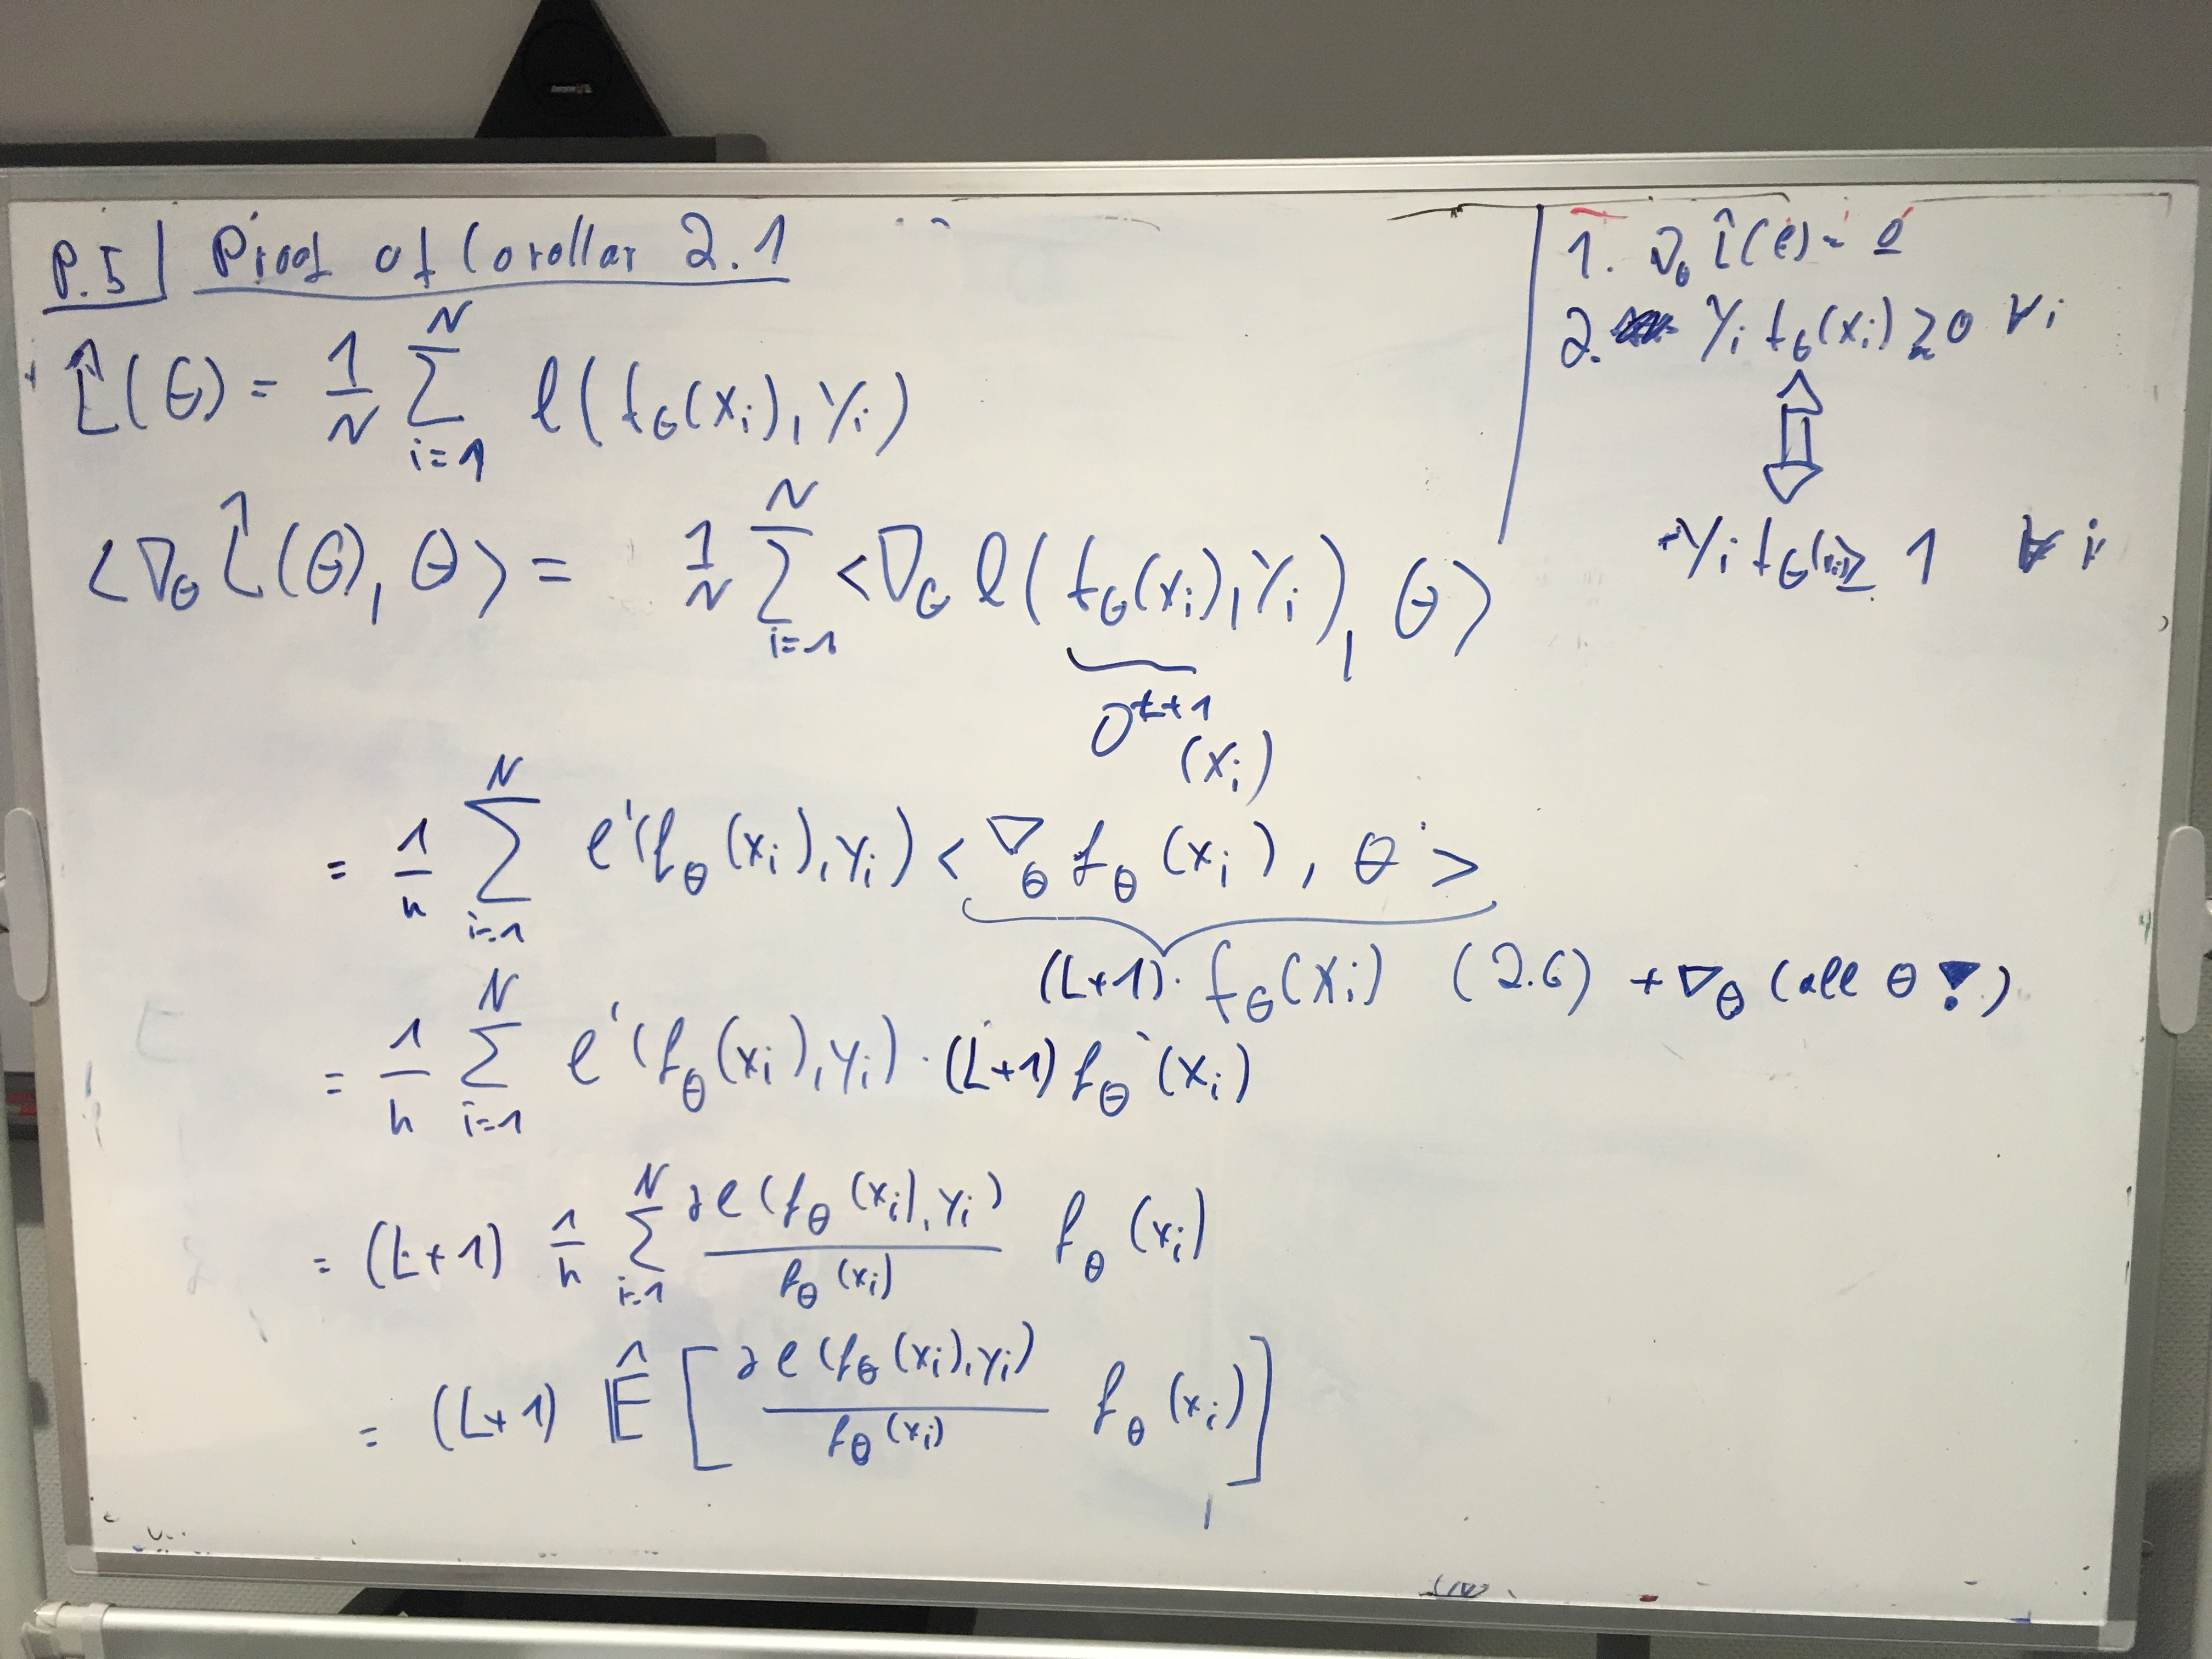
\includegraphics[width=\textwidth]{whiteboard_notes/05.jpg}
\end{figure}
\begin{figure}[htb]
	\centering
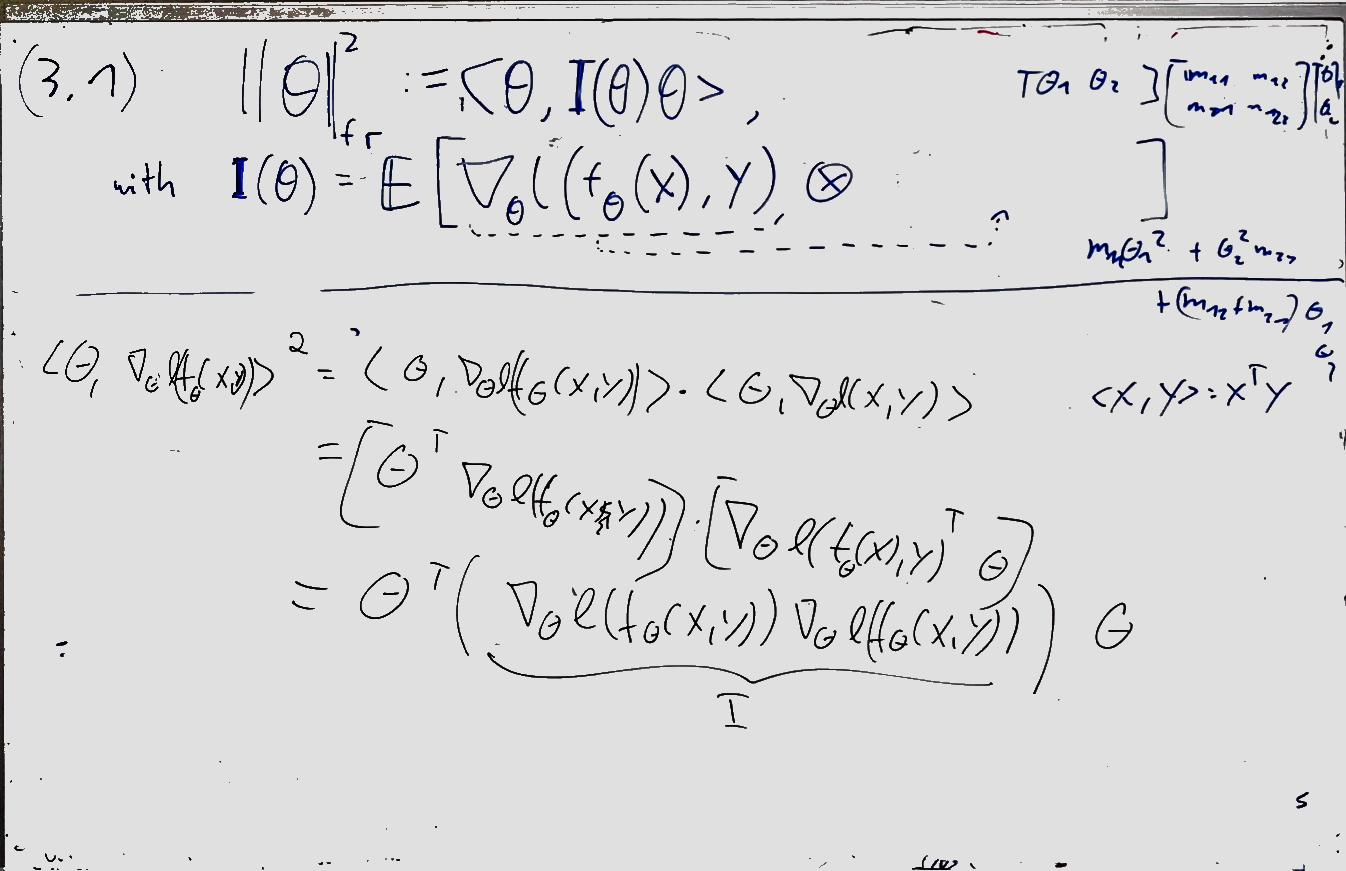
\includegraphics[width=\textwidth]{whiteboard_notes/3_1_proof.jpg}
\end{figure}

\begin{figure}[htb]
	\centering
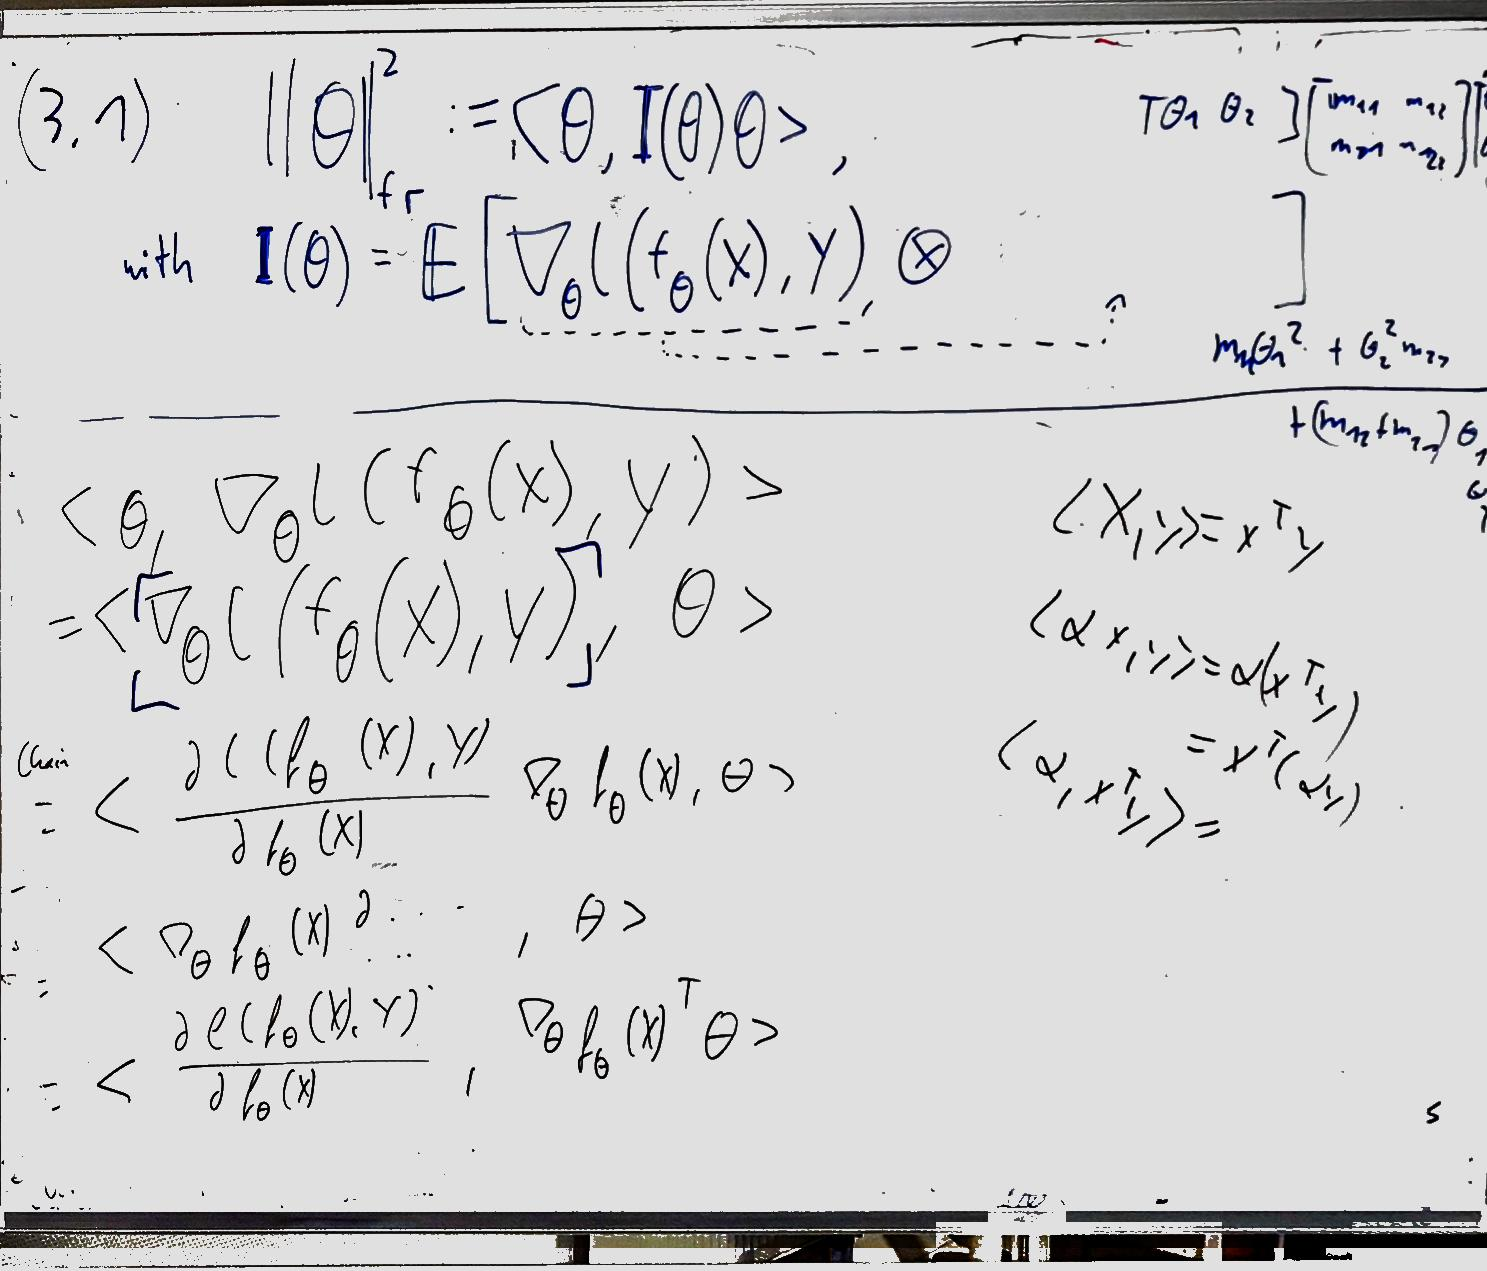
\includegraphics[width=\textwidth]{whiteboard_notes/3_1_proof_cont.jpg}
\end{figure}

\begin{figure}[htb]
	\centering
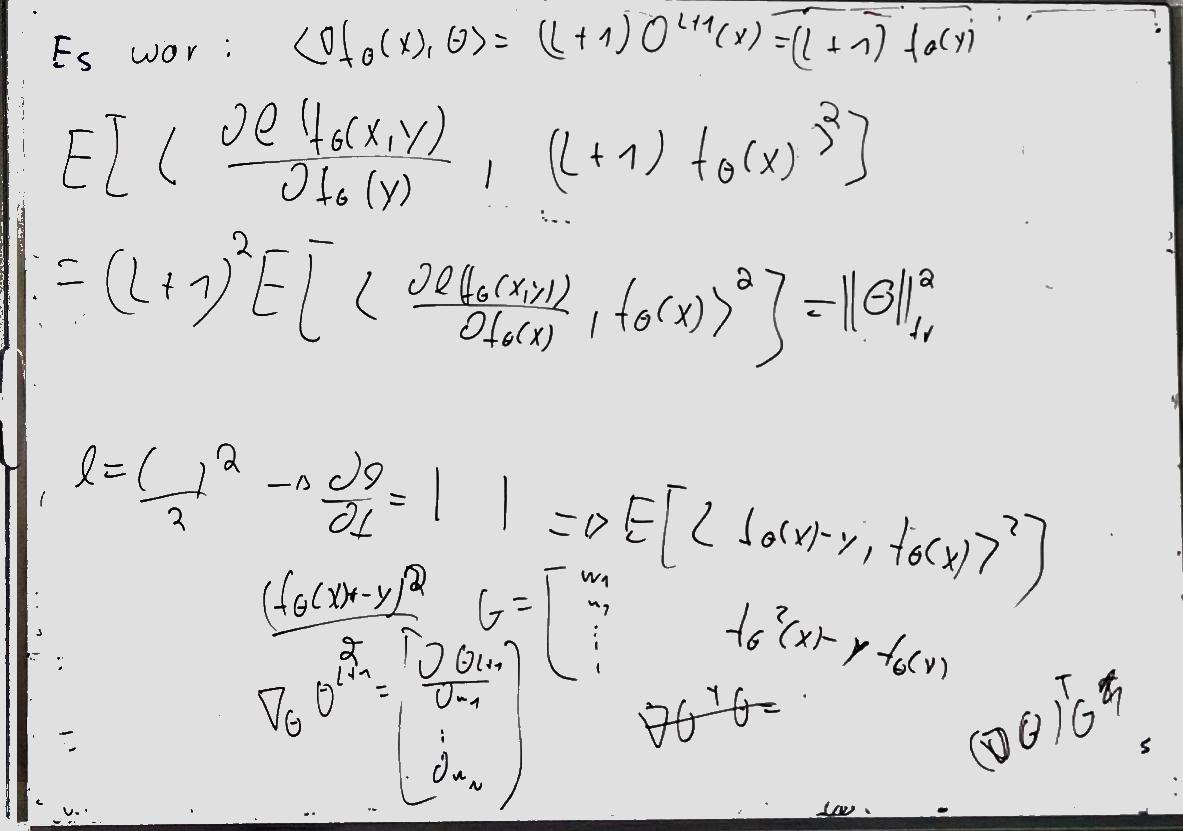
\includegraphics[width=\textwidth]{whiteboard_notes/07.jpg}
\end{figure}

\begin{figure}[htb]
	\centering
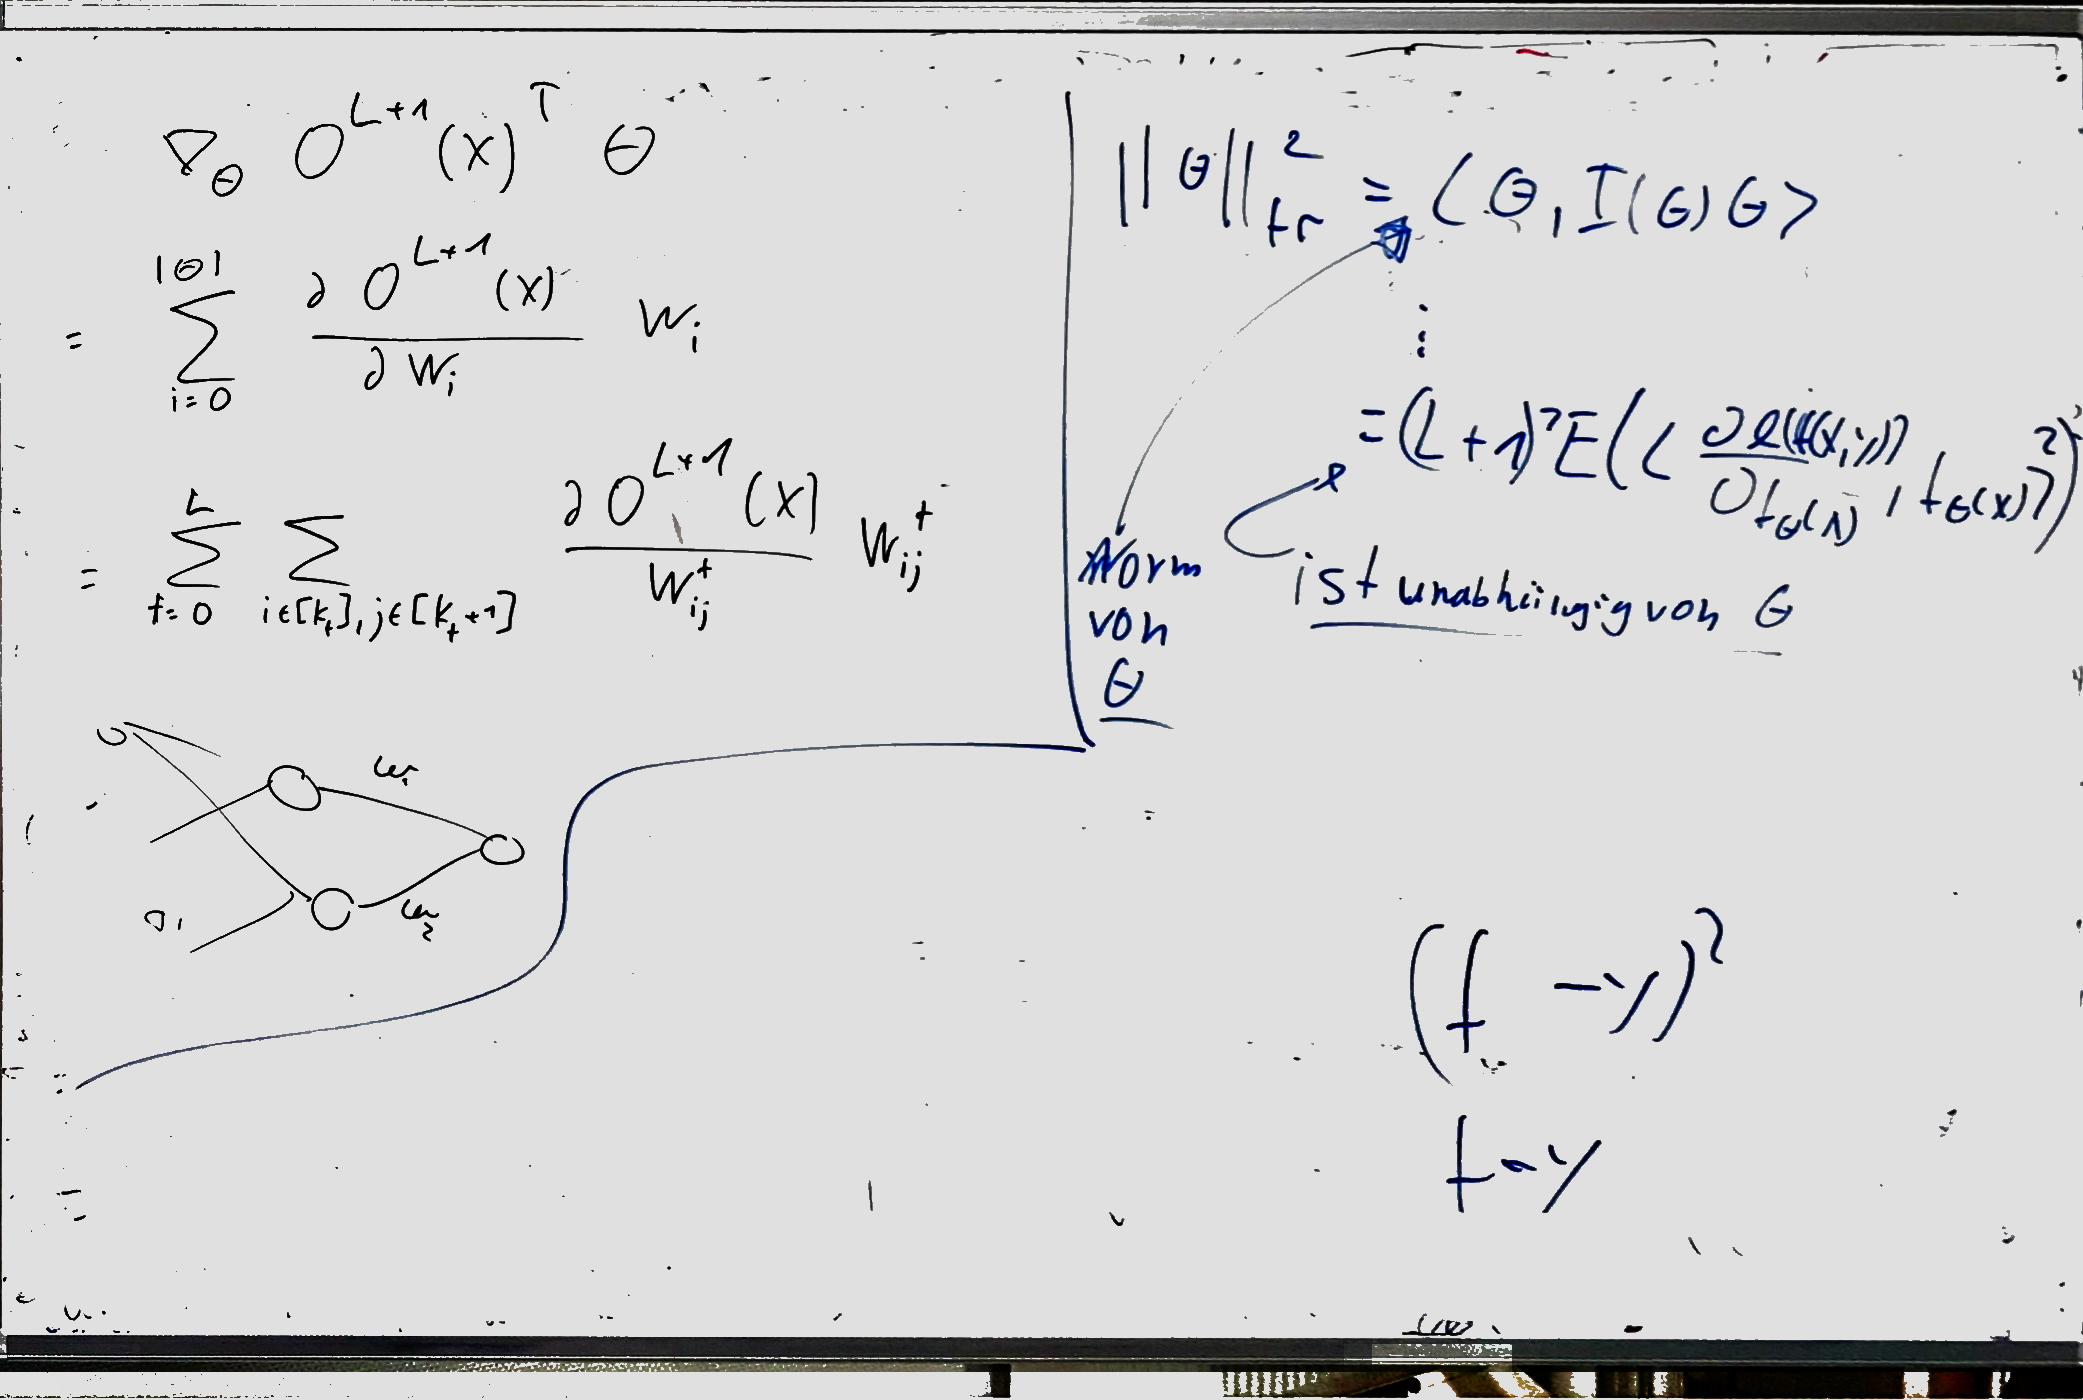
\includegraphics[width=\textwidth]{whiteboard_notes/08.jpg}
\end{figure}

\begin{figure}[htb]
	\centering
	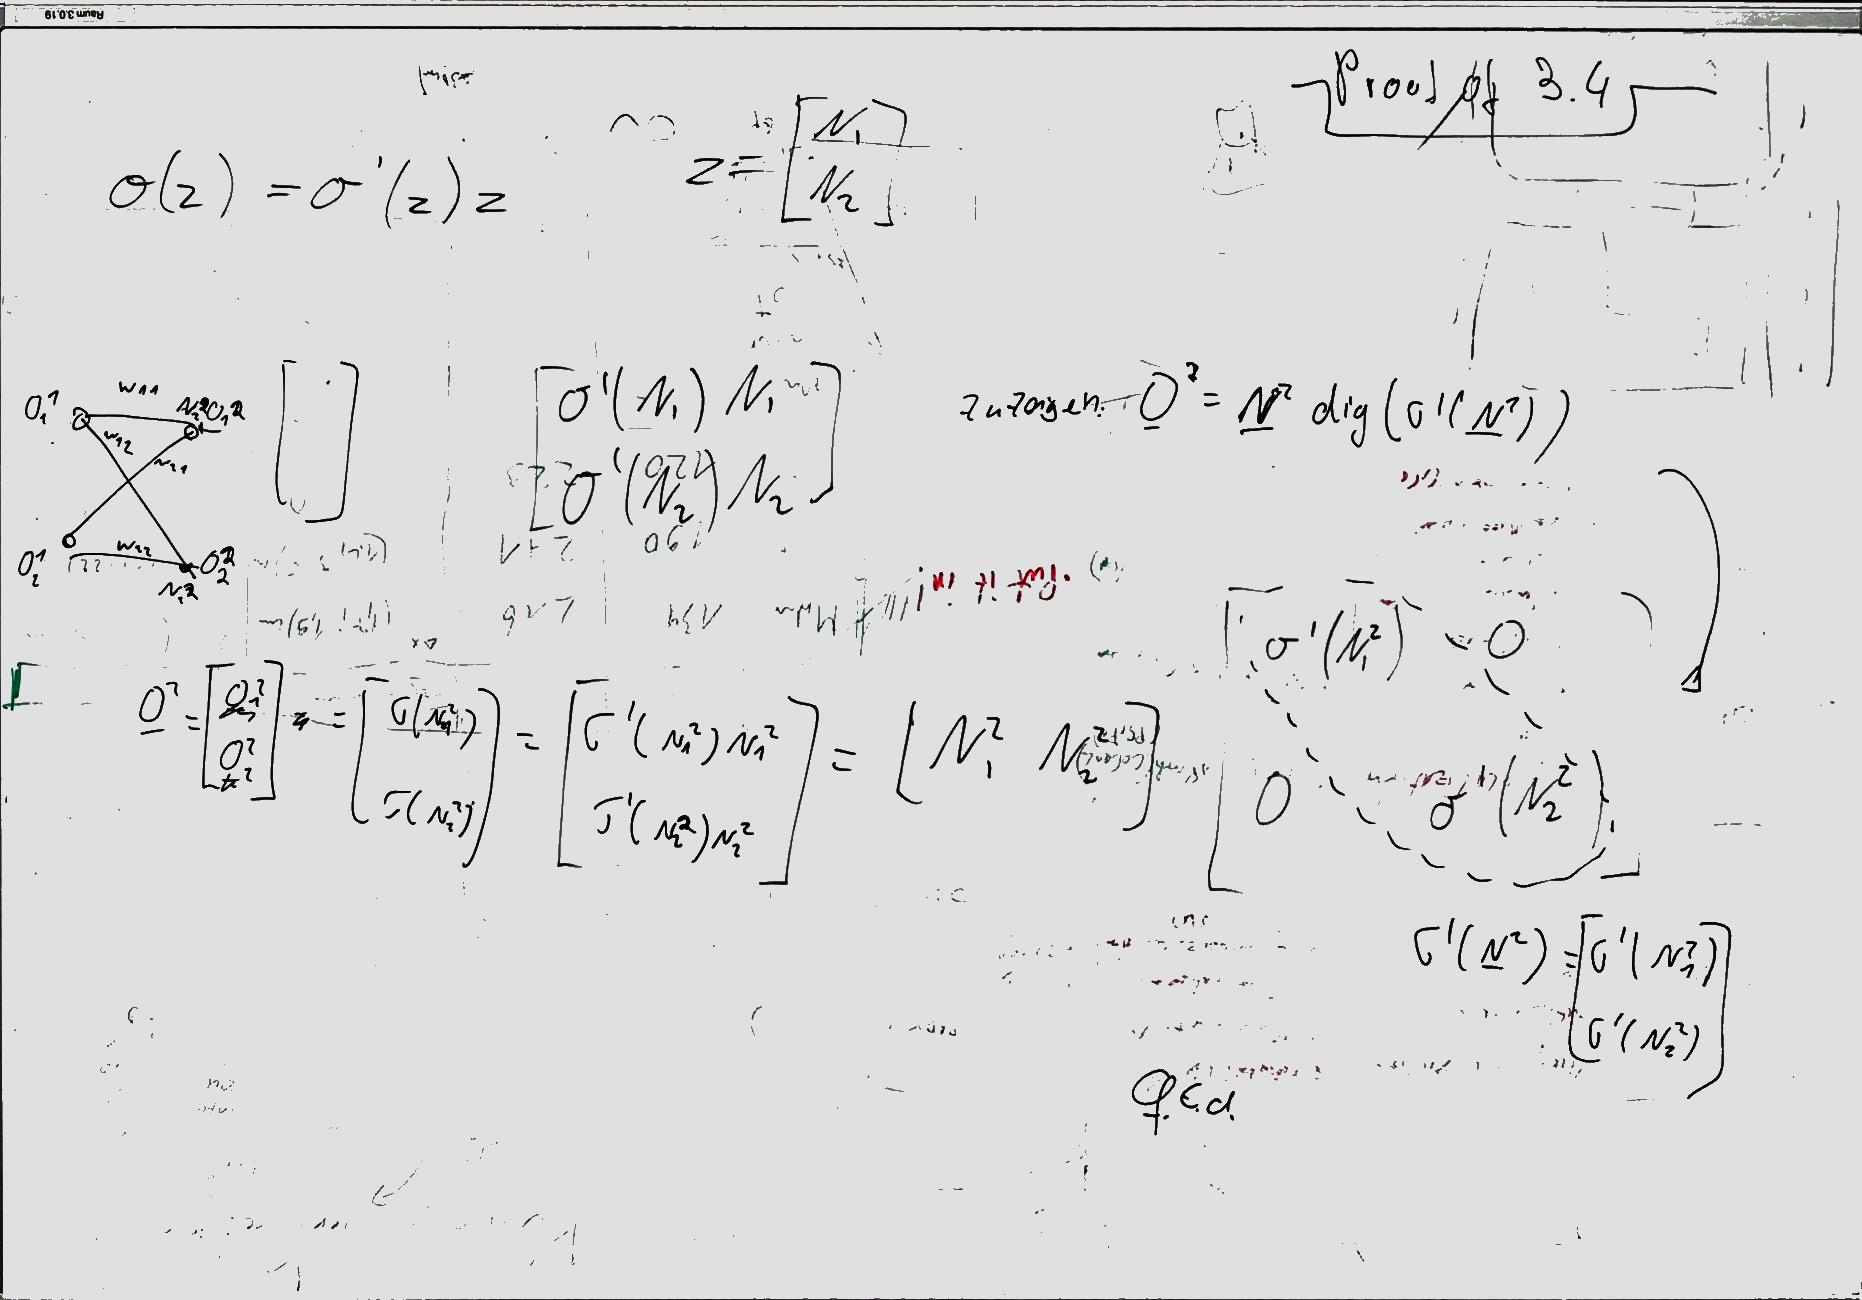
\includegraphics[width=\textwidth]{whiteboard_notes/09.jpg}
\end{figure}

\begin{figure}[htb]
	\centering
	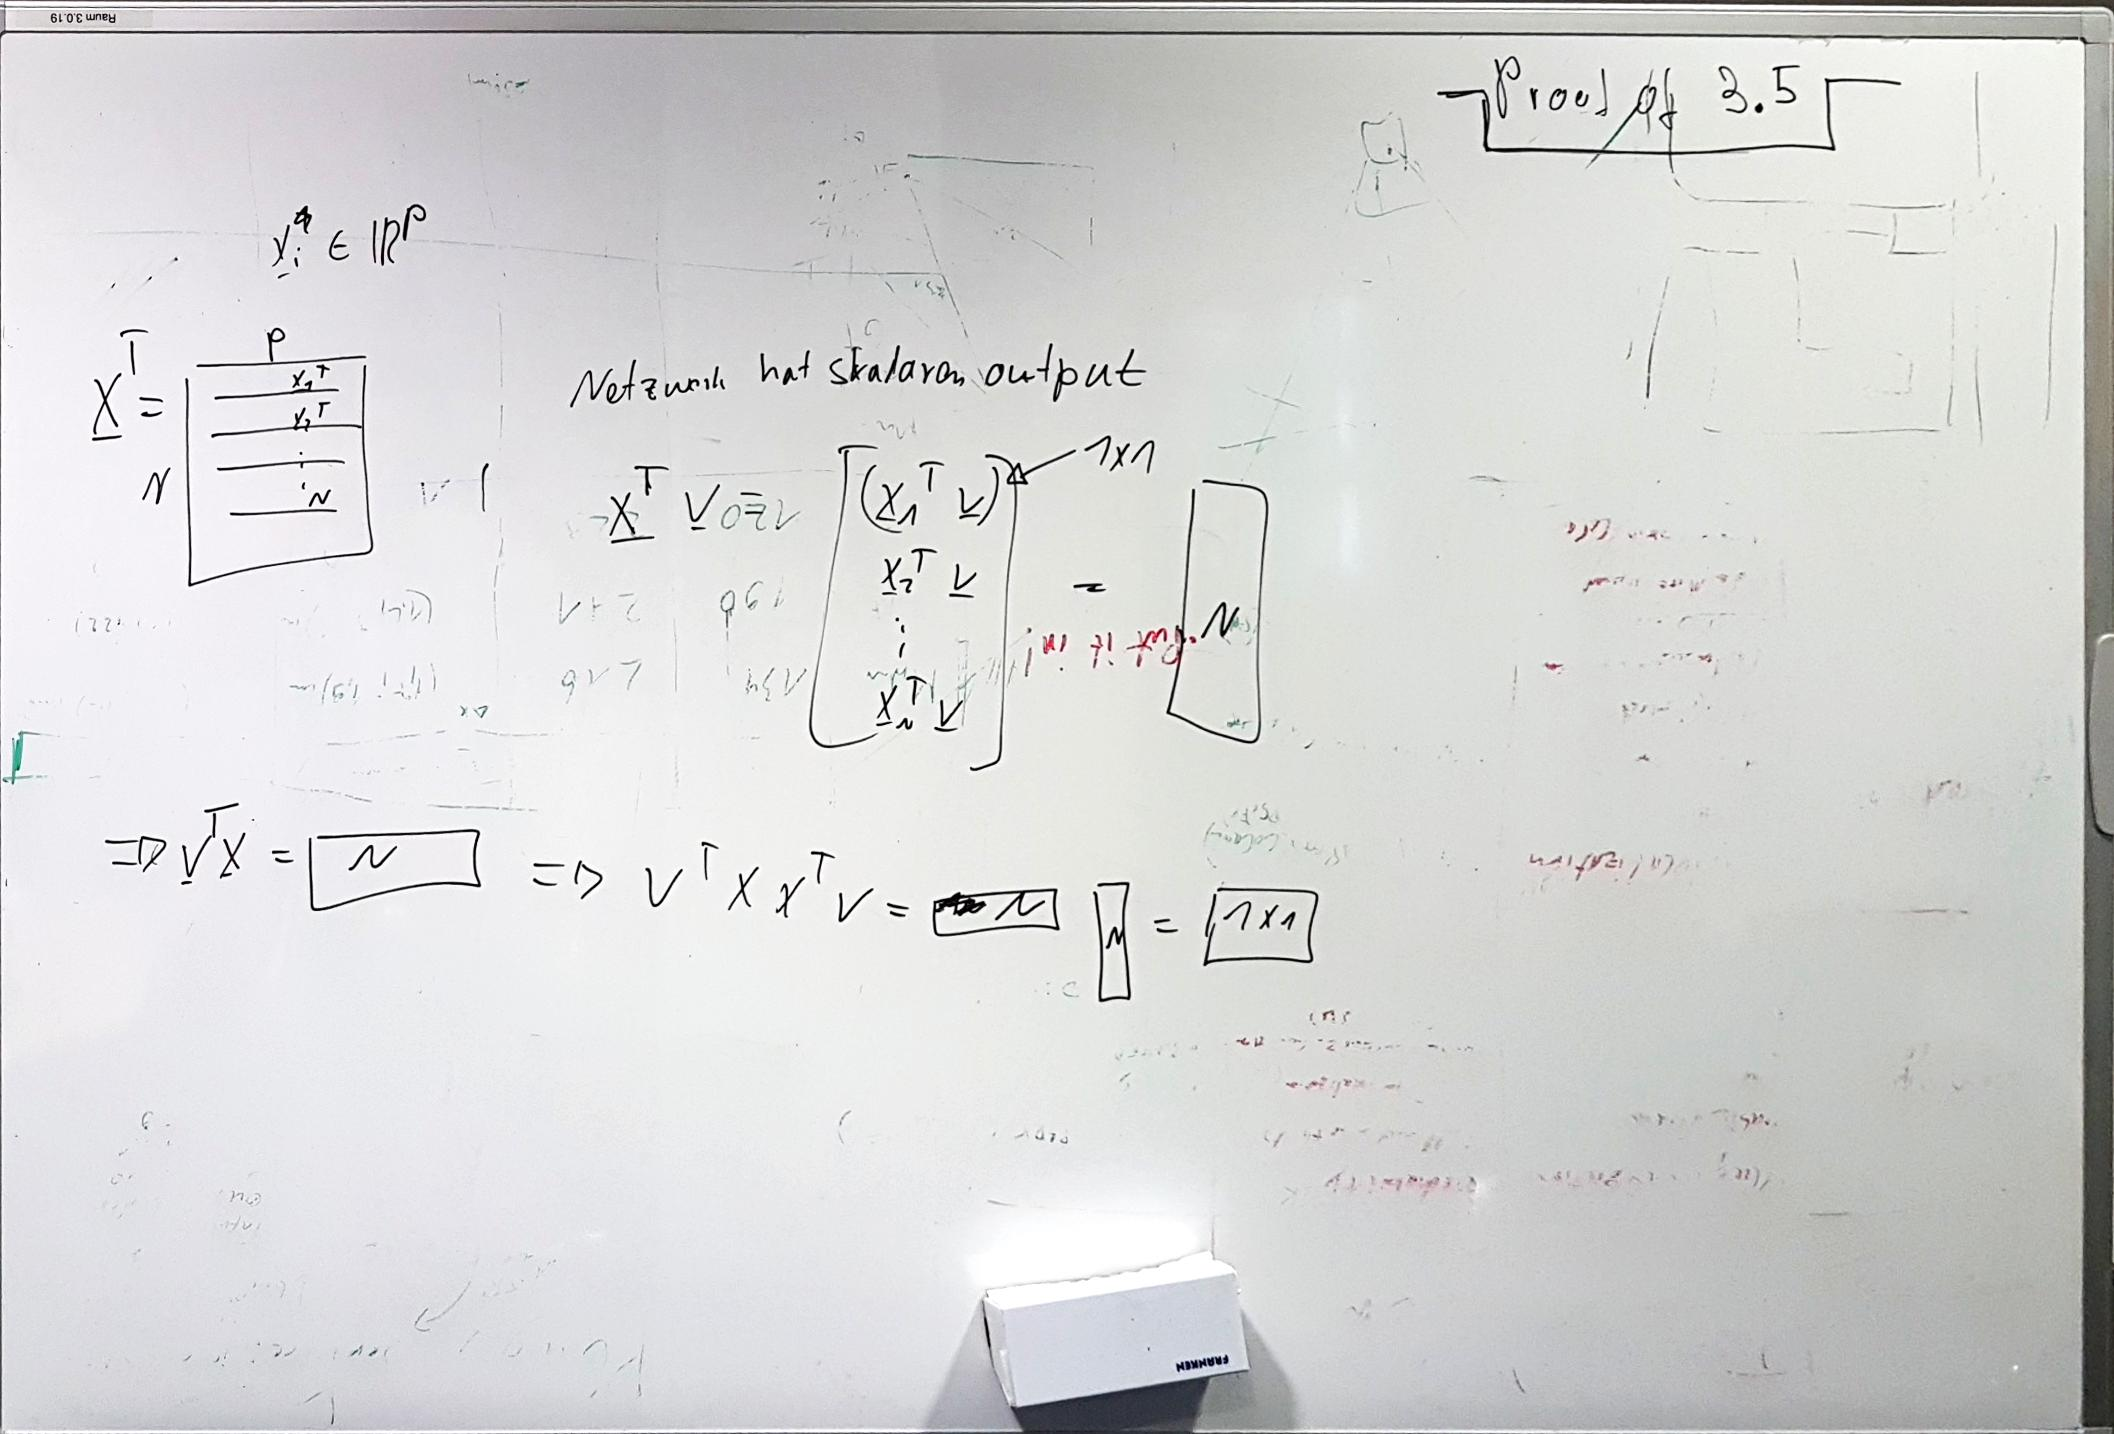
\includegraphics[width=\textwidth]{whiteboard_notes/10.jpg}
\end{figure}

\begin{figure}[htb]
	\centering
	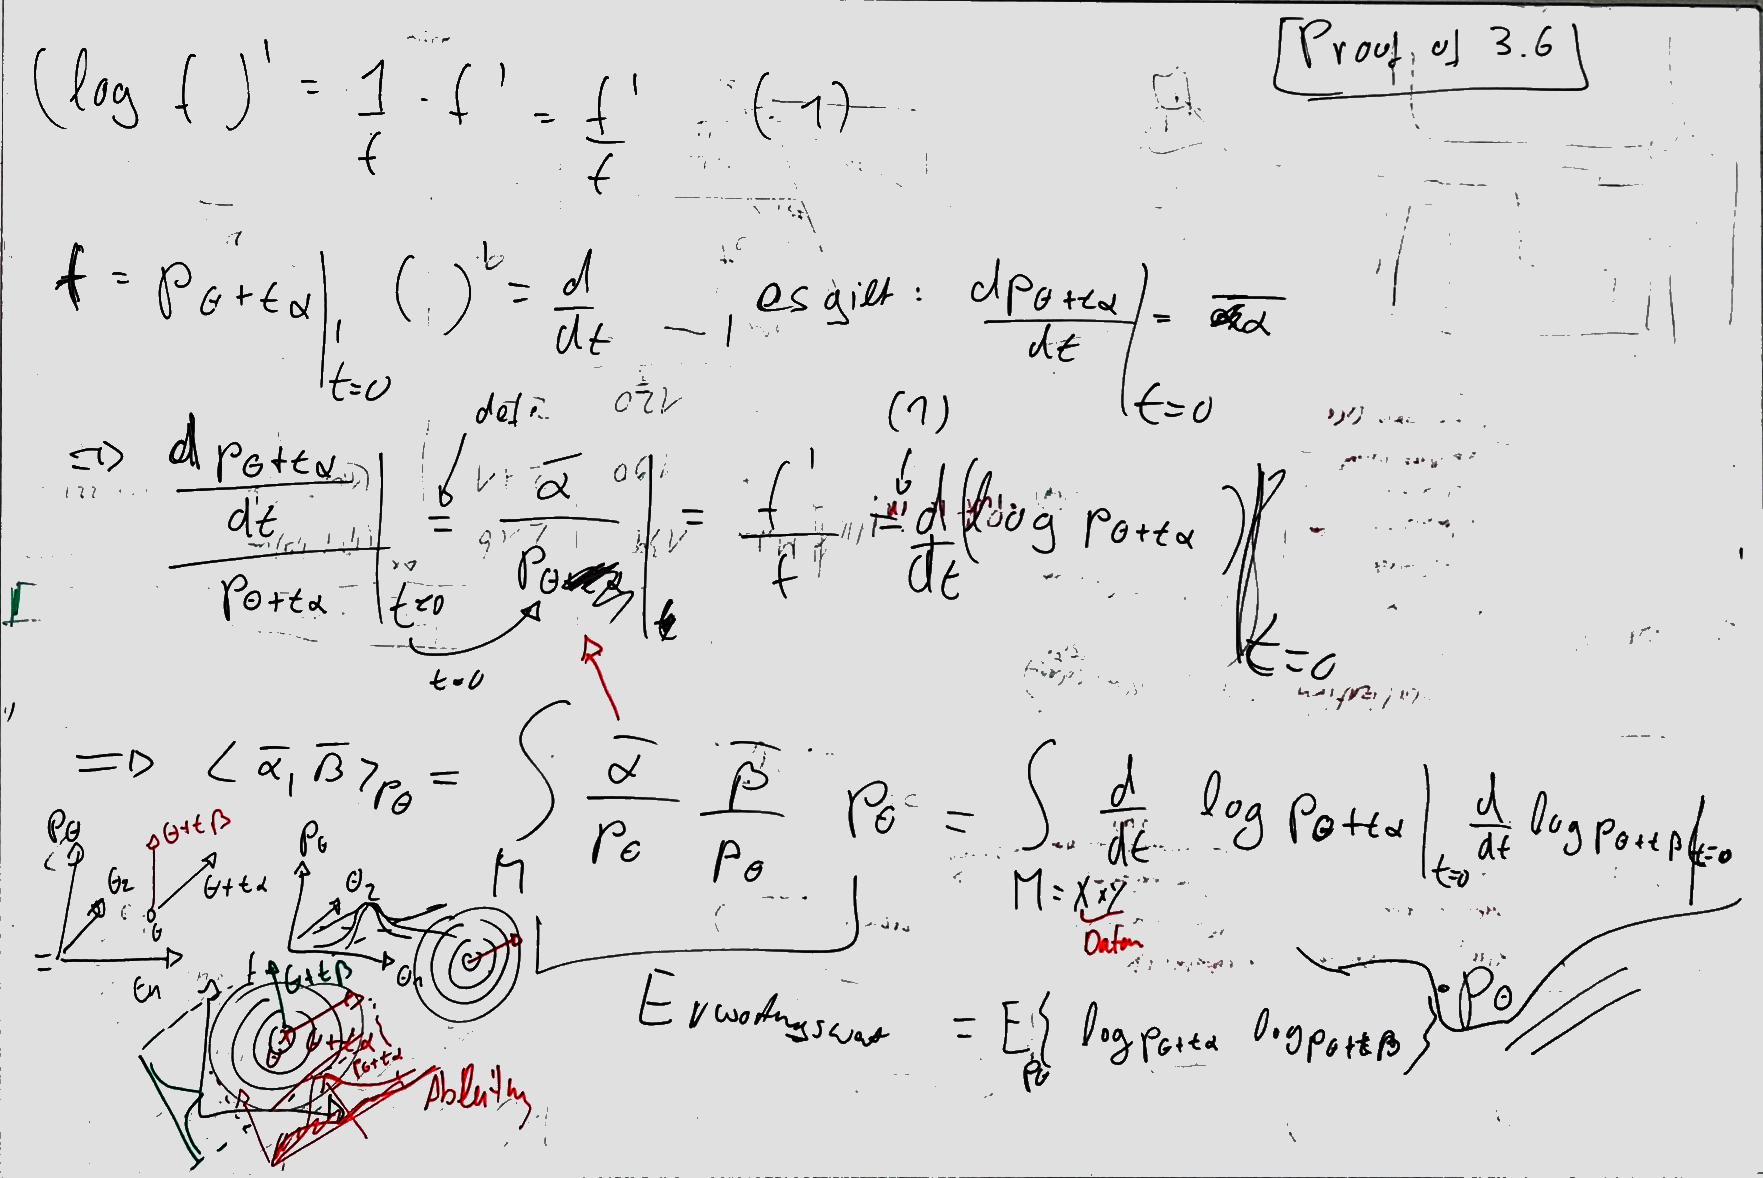
\includegraphics[width=\textwidth]{whiteboard_notes/11.jpg}
\end{figure}

\begin{figure}[htb]
	\centering
	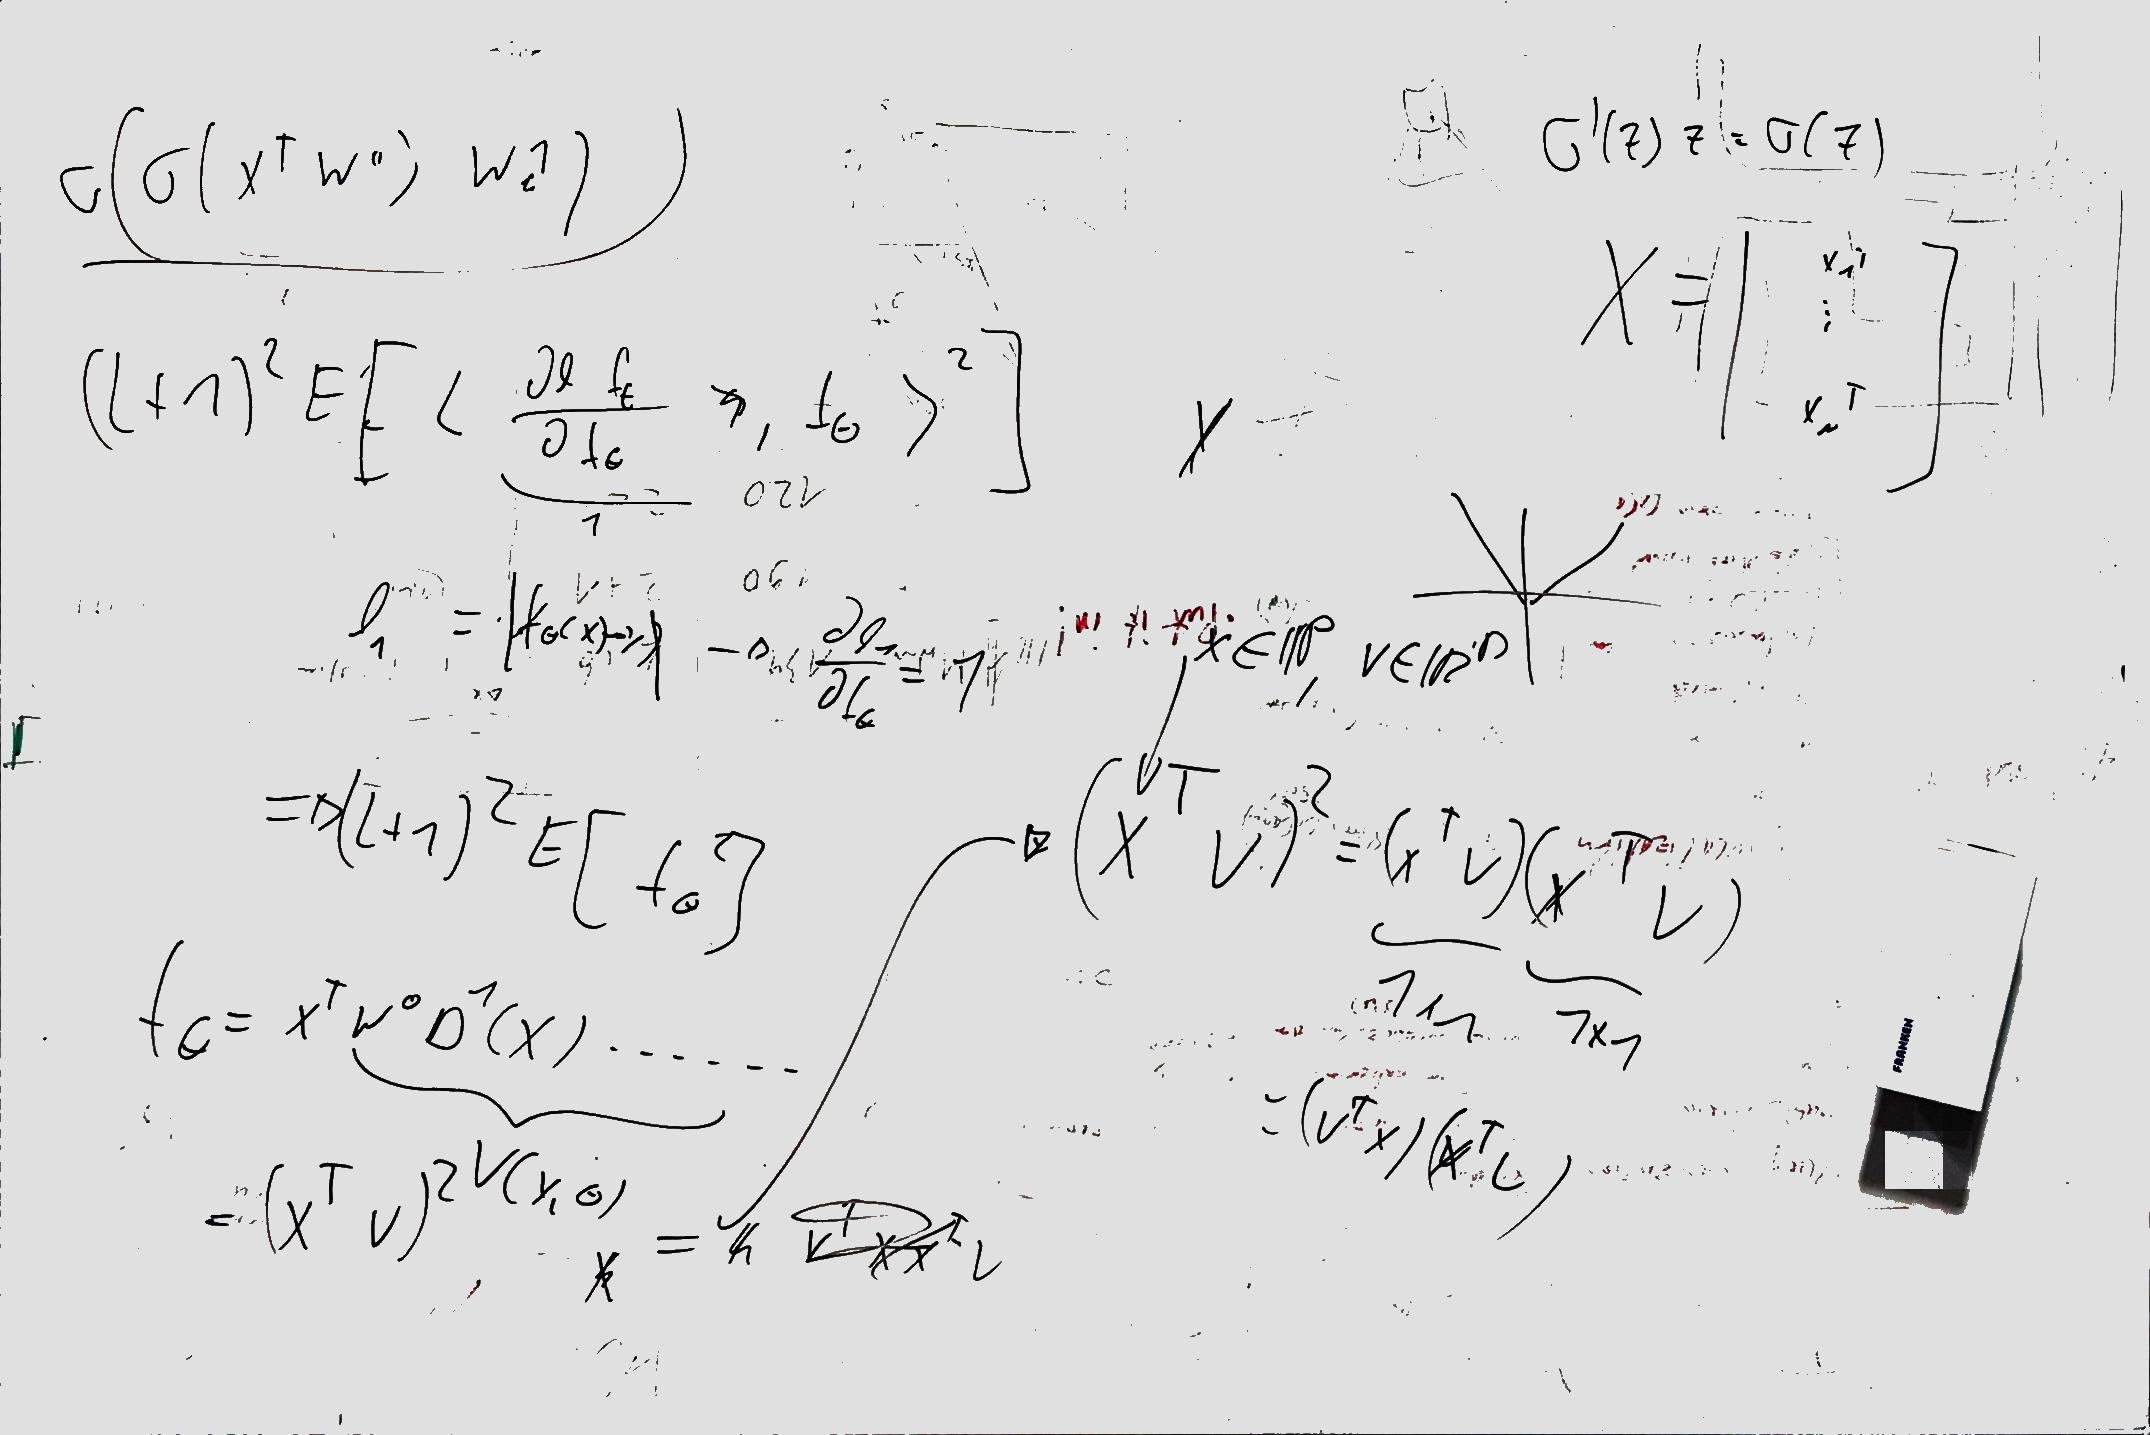
\includegraphics[width=\textwidth]{whiteboard_notes/12.jpg}
\end{figure}

\begin{figure}[htb]
	\centering
	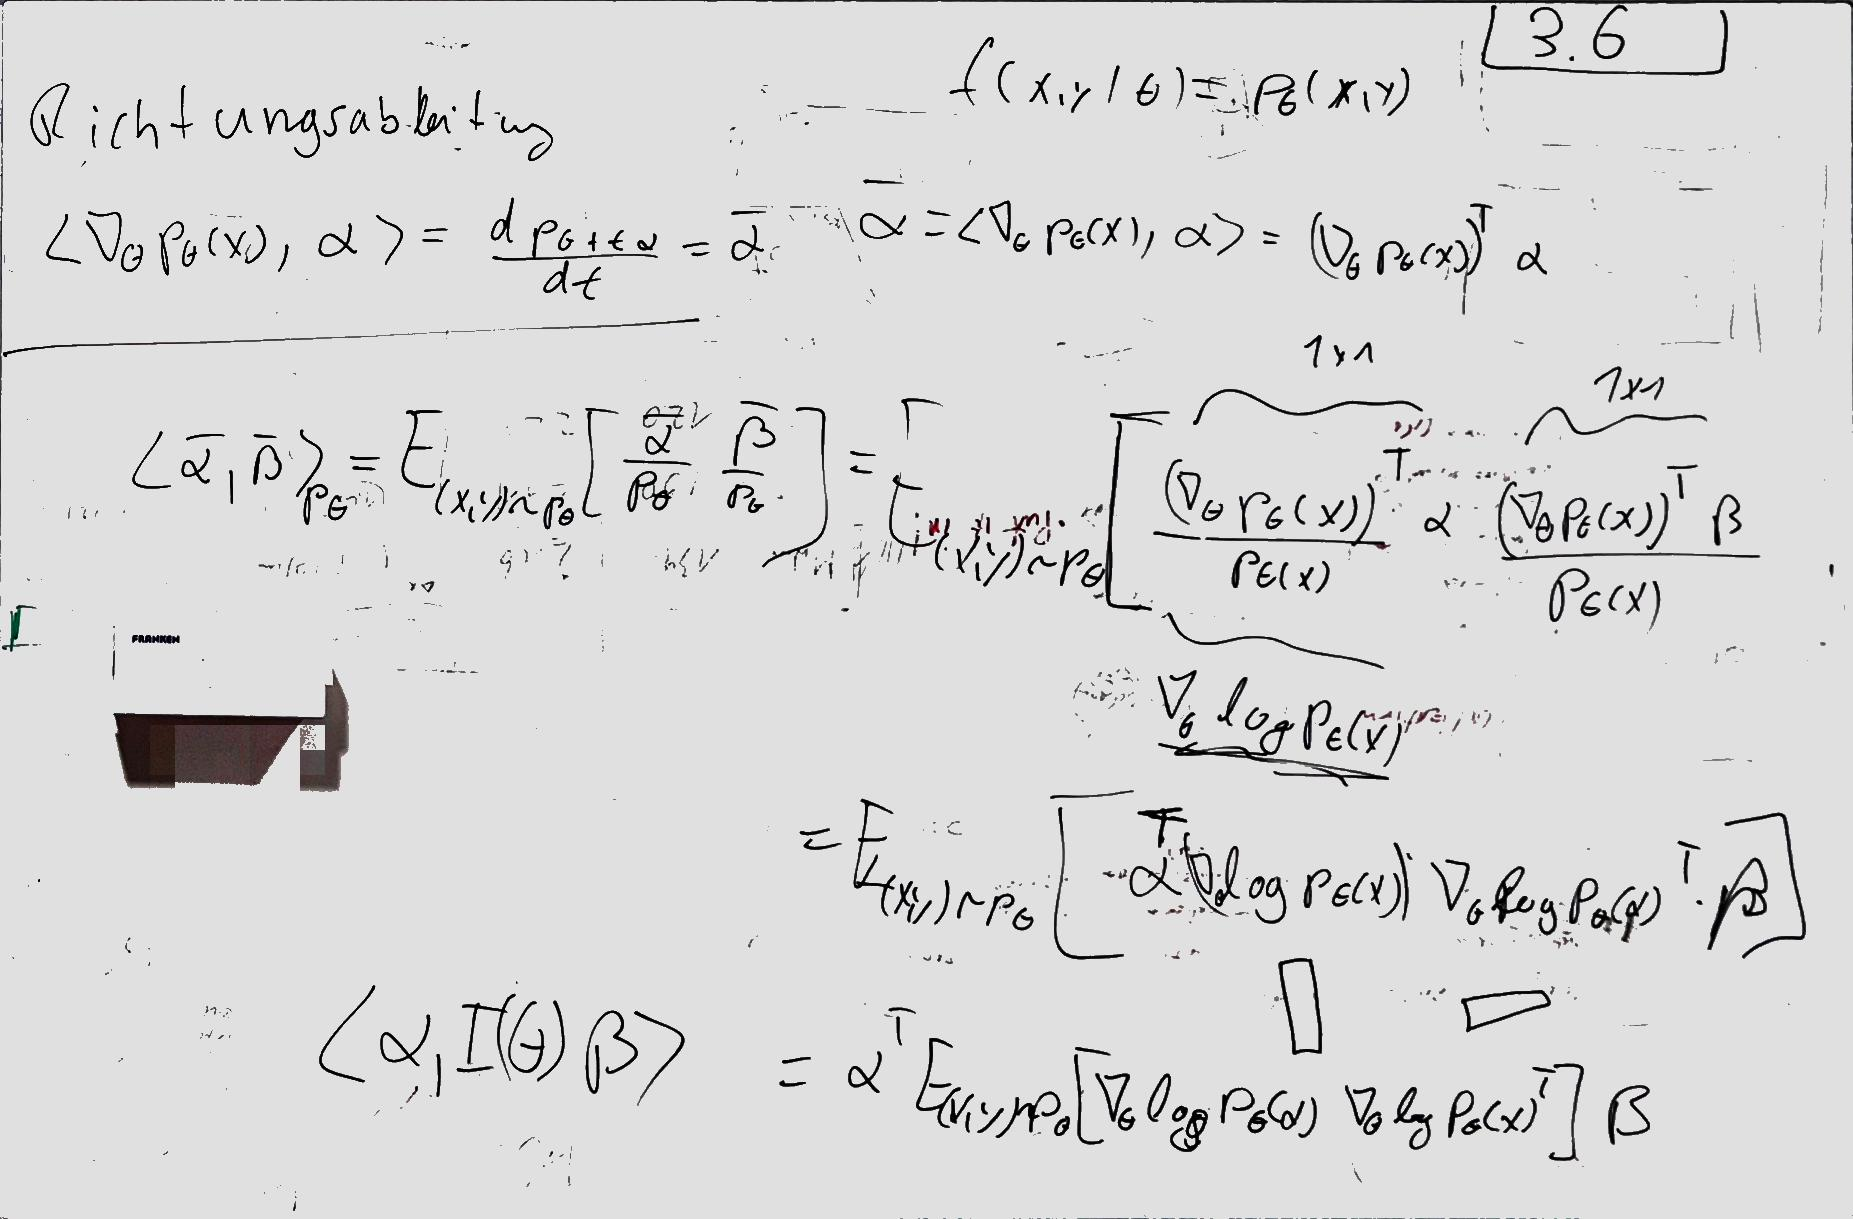
\includegraphics[width=\textwidth]{whiteboard_notes/13.jpg}
\end{figure}

\begin{figure}[htb]
	\centering
	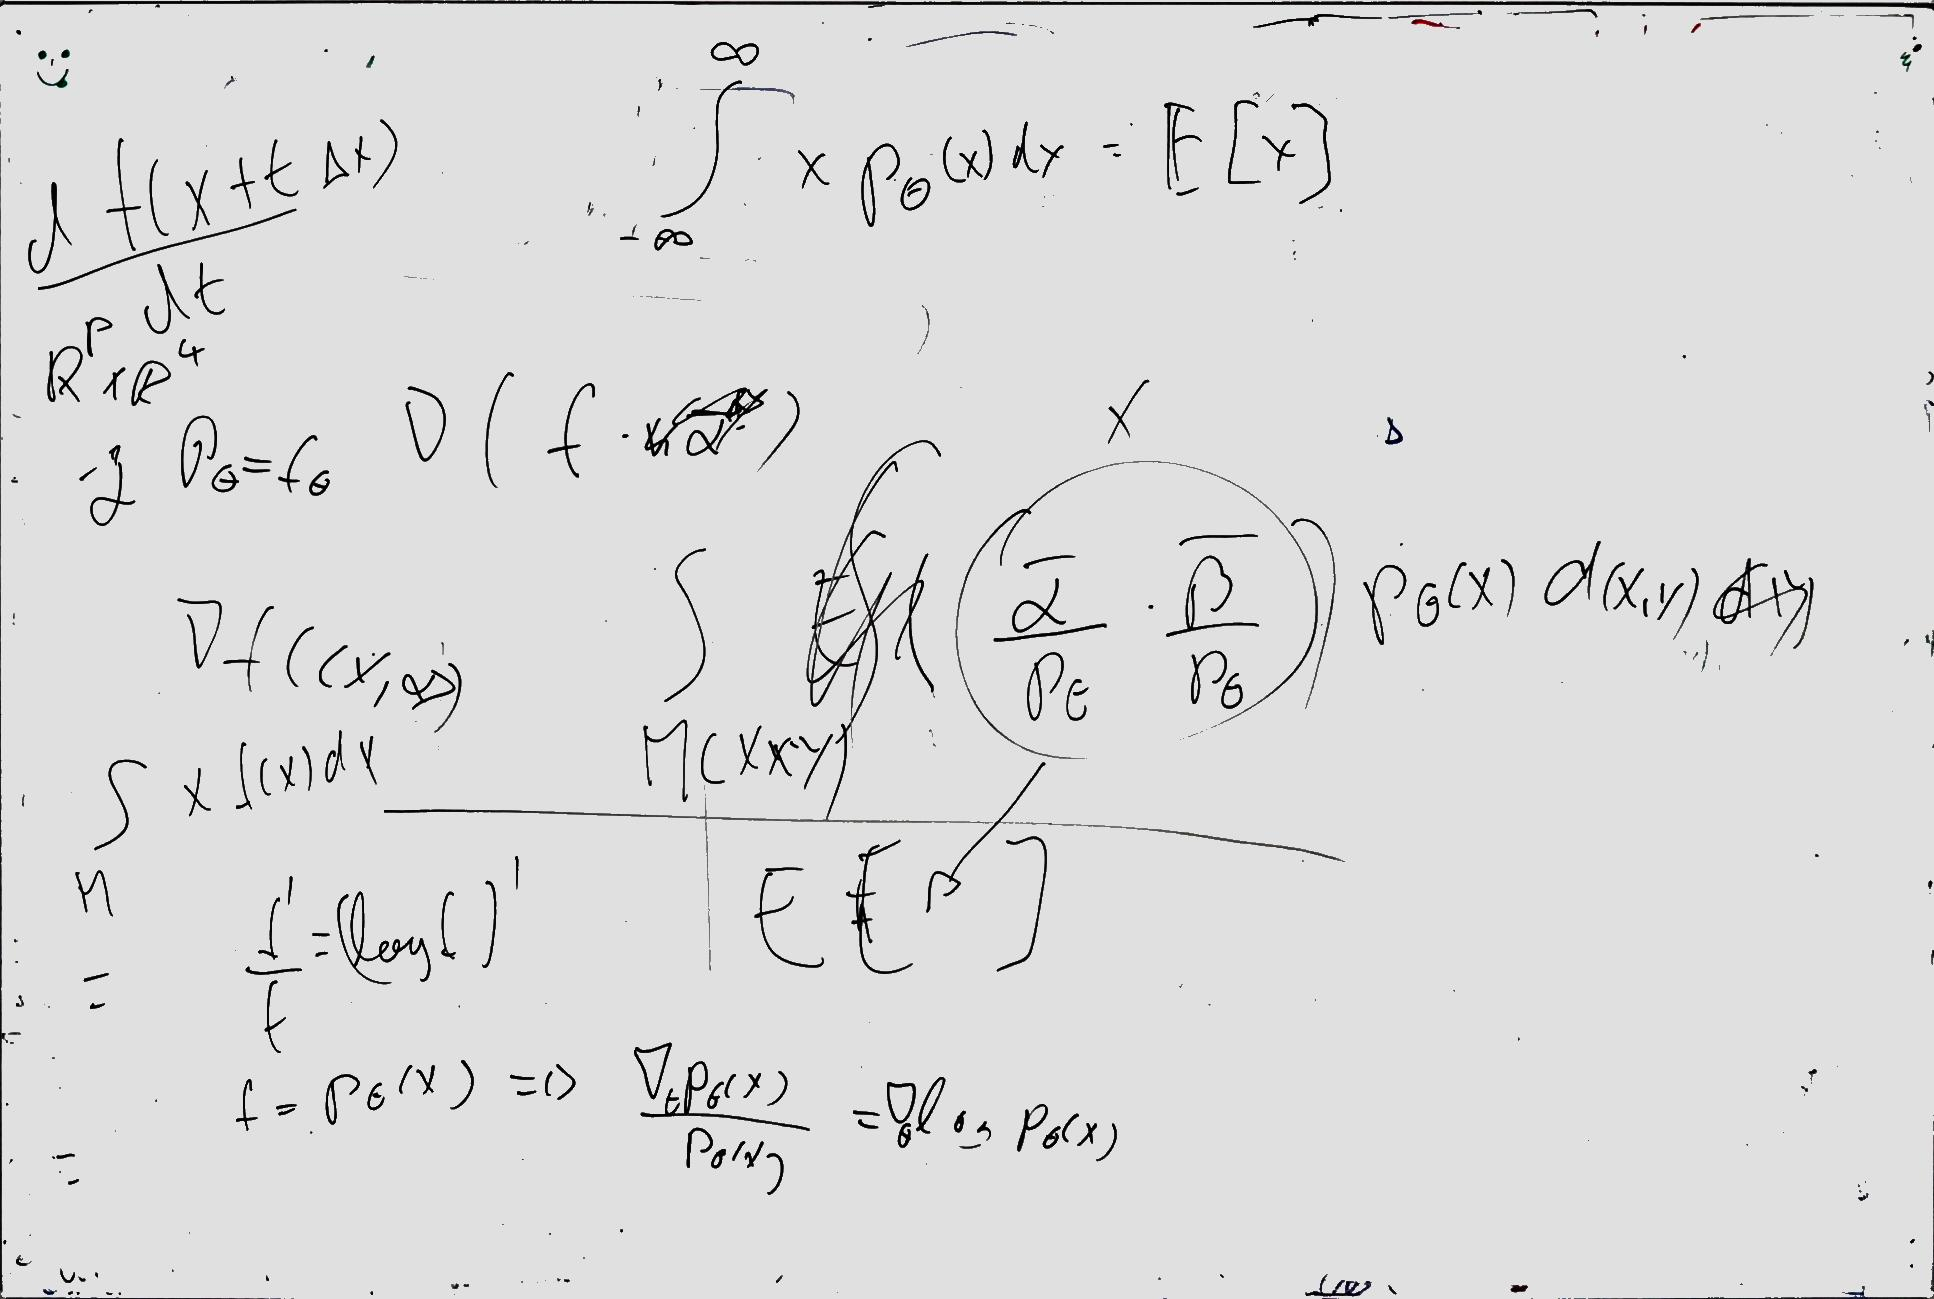
\includegraphics[width=\textwidth]{whiteboard_notes/14.jpg}
\end{figure}

\begin{figure}[htb]
	\centering
	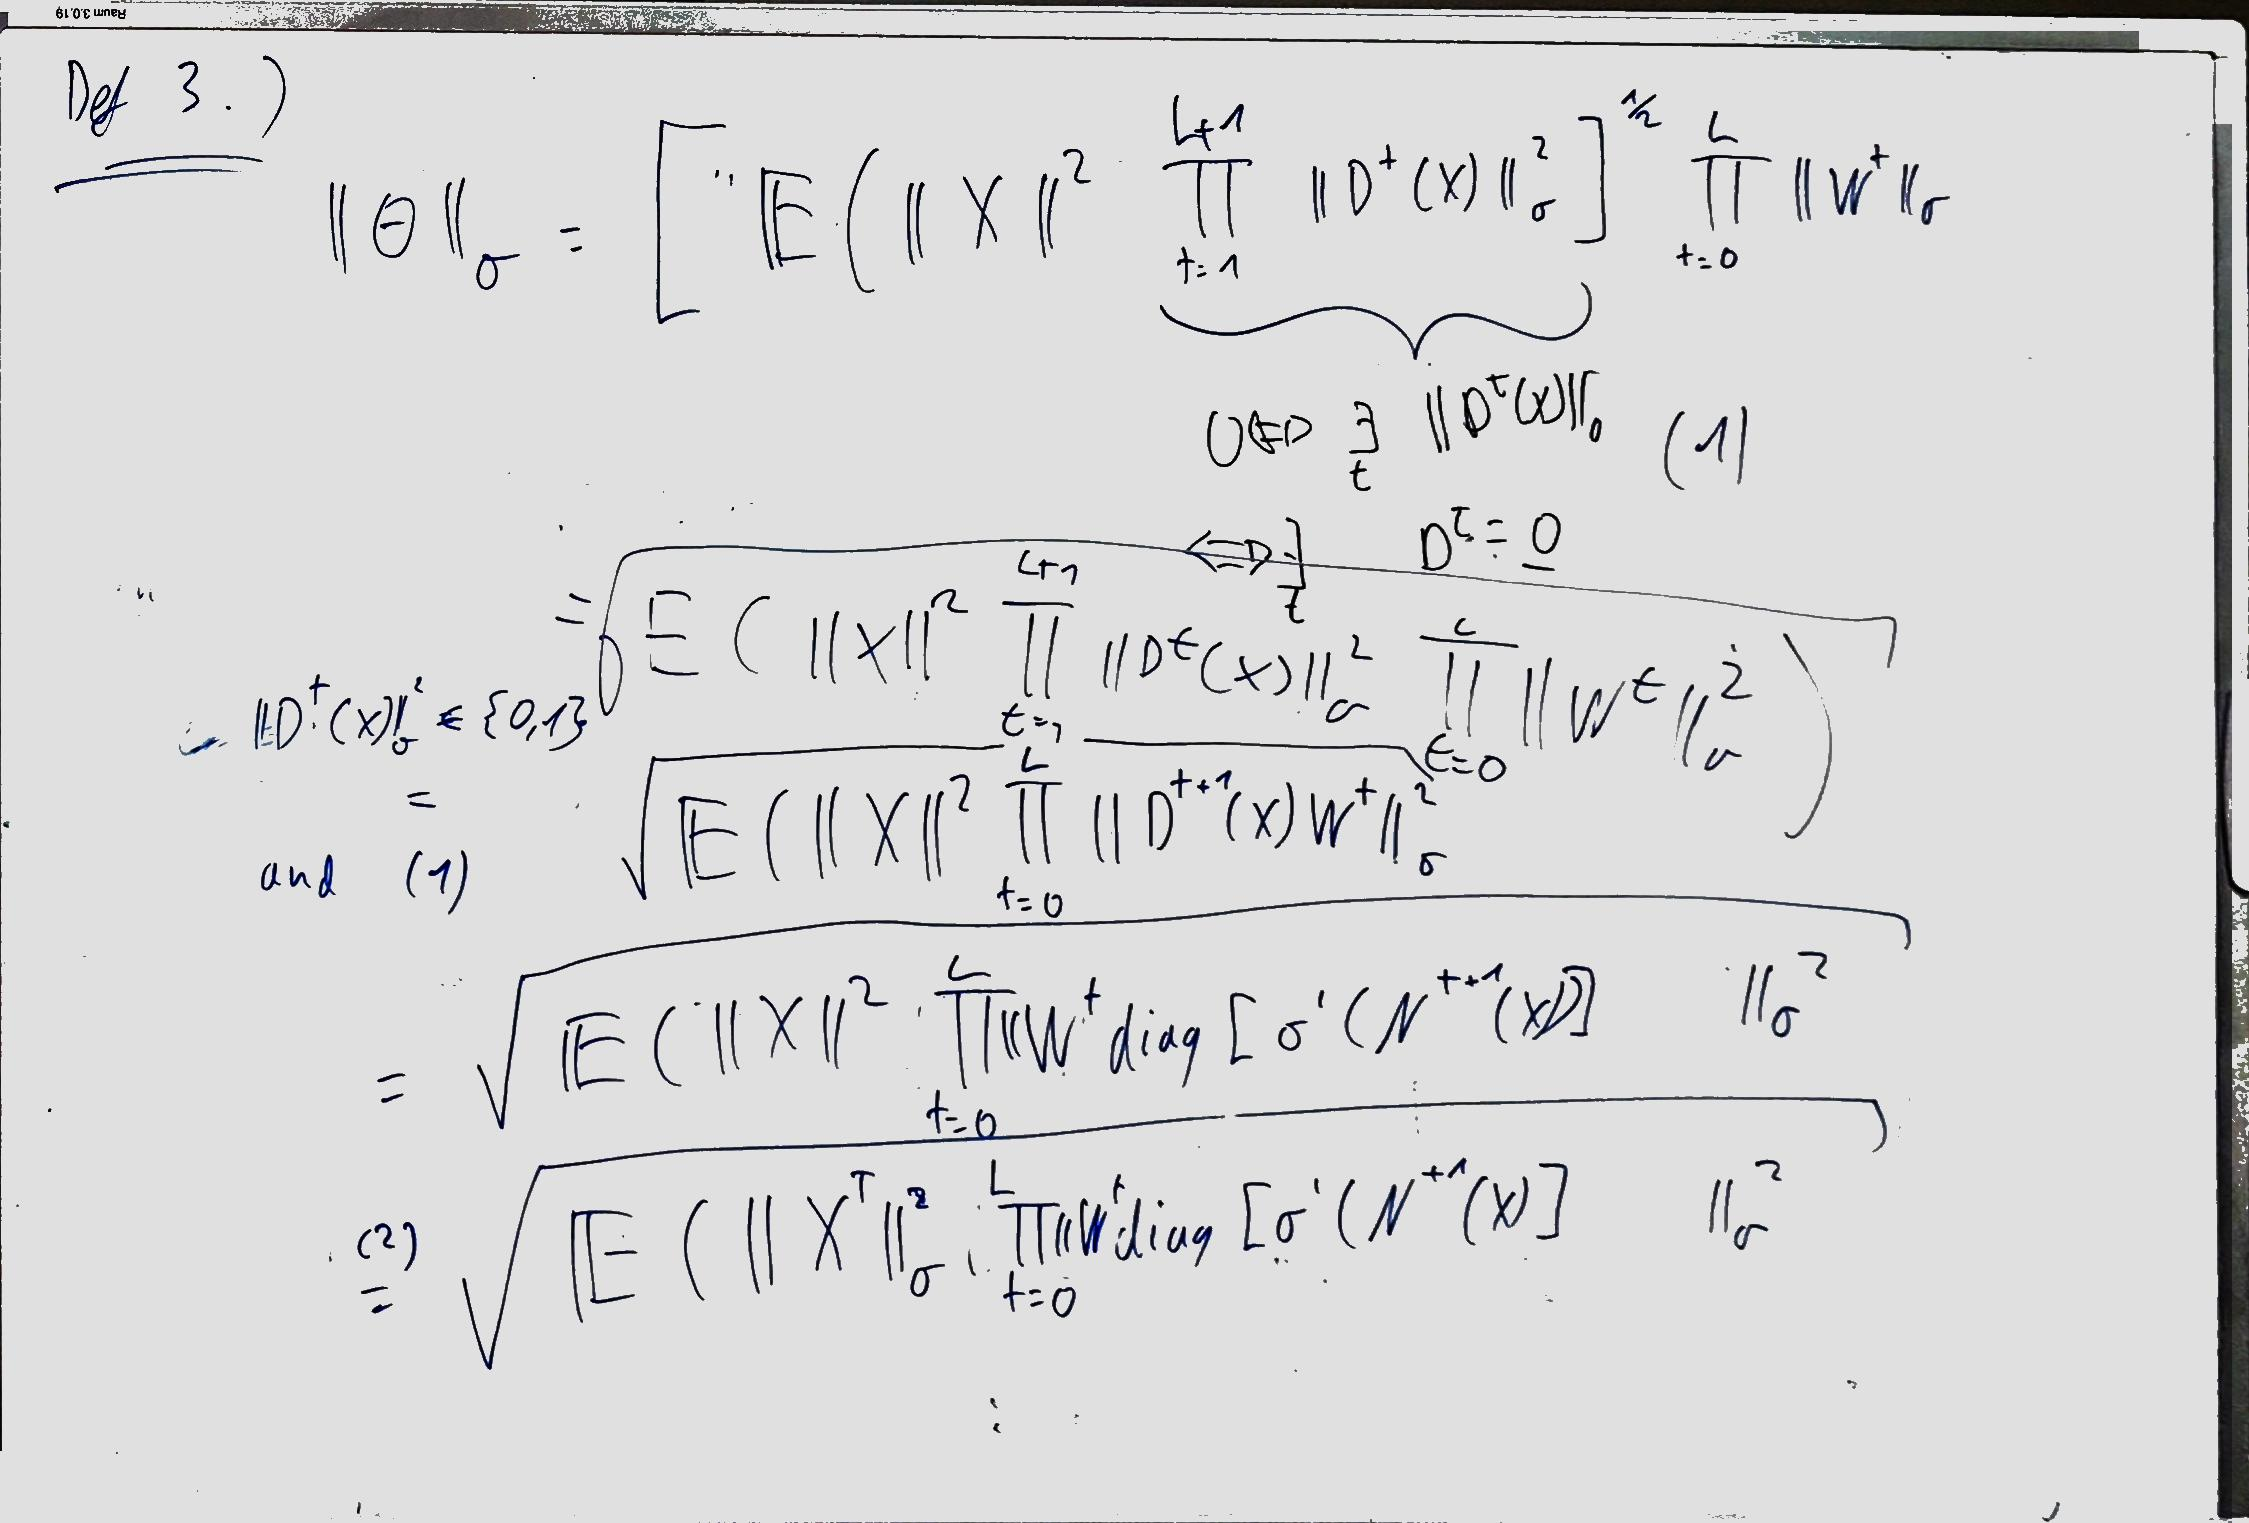
\includegraphics[width=\textwidth]{whiteboard_notes/15.jpg}
\end{figure}

\begin{figure}[htb]
	\centering
	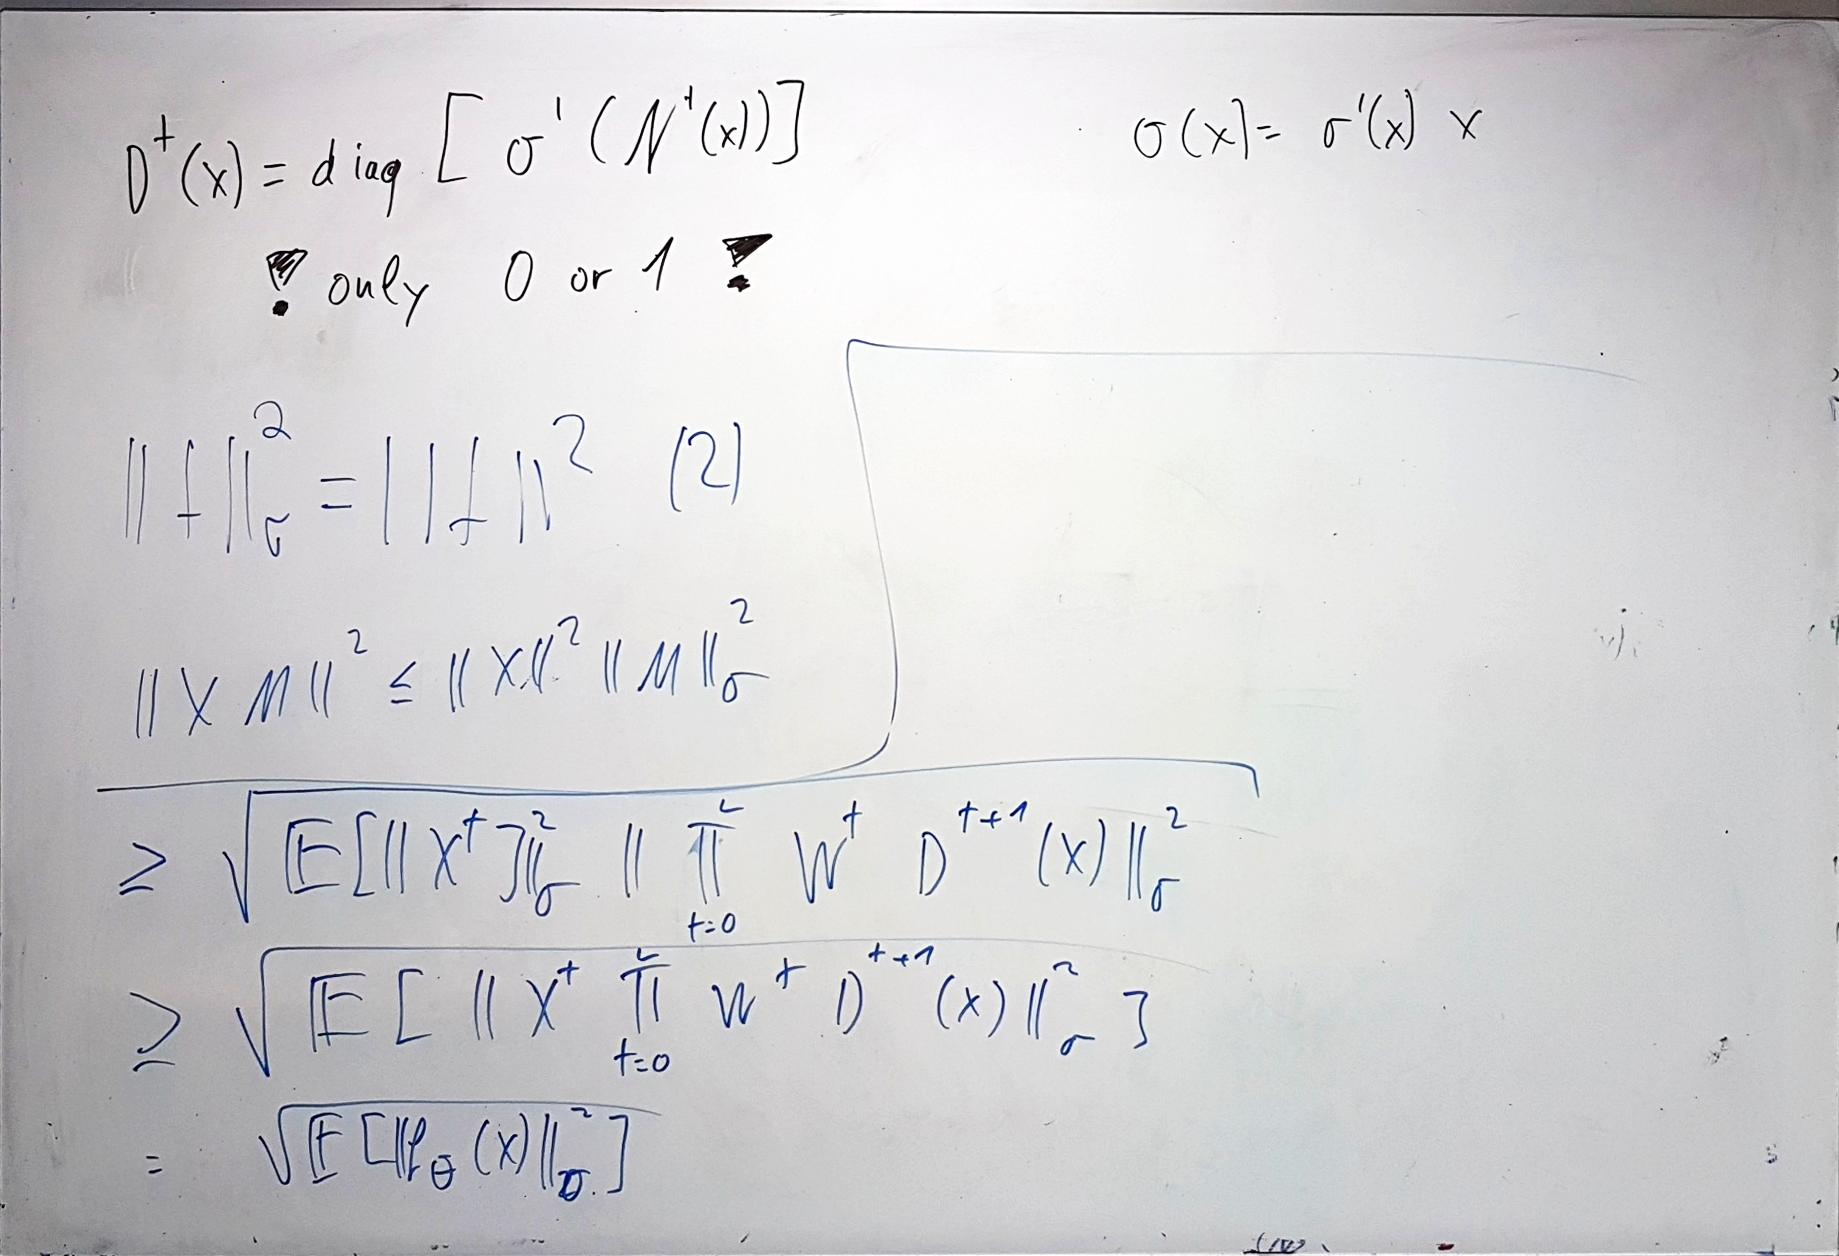
\includegraphics[width=\textwidth]{whiteboard_notes/16.jpg}
\end{figure}

\begin{figure}[htb]
	\centering
	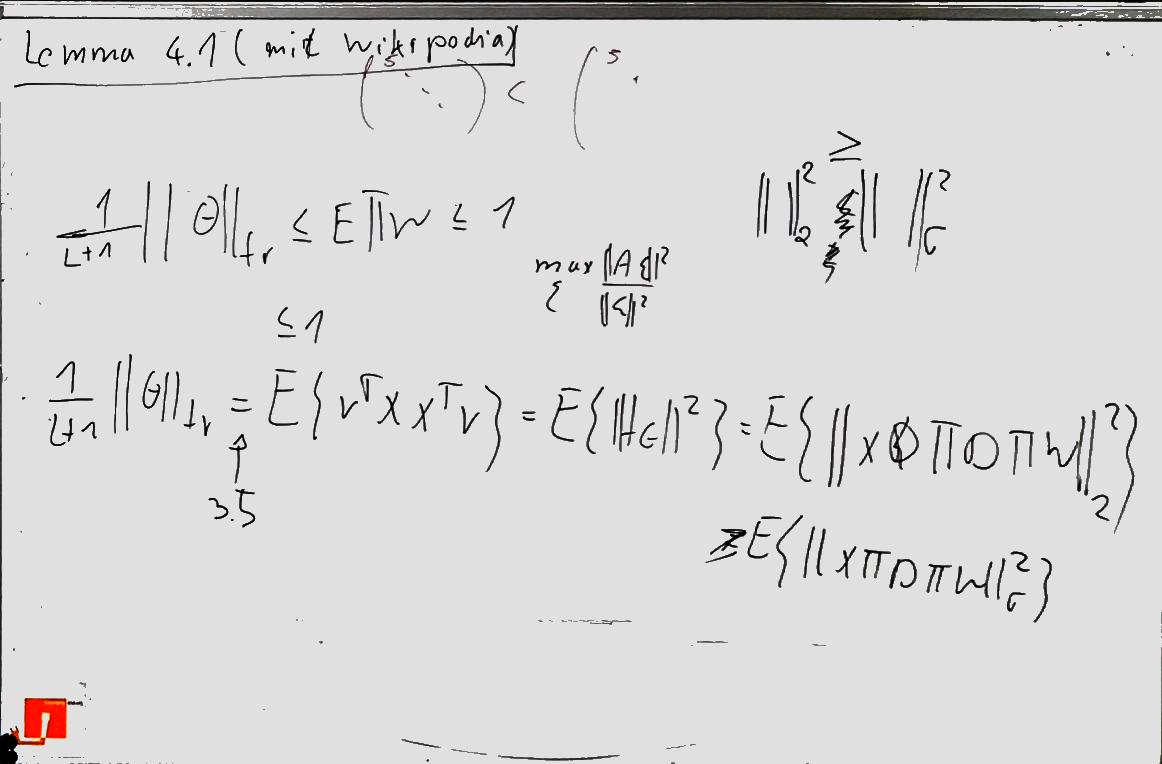
\includegraphics[width=\textwidth]{whiteboard_notes/17.jpg}
\end{figure}

\newpage
\section{Notes on Section 4}

\subsubsection{Explaining Lemma 4.1}

A proof of Lemma 4.1 can also be found in the appendix of the original paper. However,
the relation between the norms is missing in the original paper - that is why we state it here again.
From 3.5 in the paper, we had:
\begin{align}
	\frac{1}{(L+1)^2} \pqnorm{\theta}{fr}{2} = \E{v^\TT X X^\TT v} = \E{\norm{f_\theta}^2}.
\end{align}
Remember that the output of the network, $f_\theta(x)$, is a vector in $\setreal^k$ of probabilities for each of the $k$ classes.  
For the Frobenius Norm of a Matrix $A$ and a vector $x$ the following holds.
\begin{align}
	\frobnorm{A} &\geq \spectralnorm{A} \\
	\frobnorm{x} &= \lnorm{x} = \spectralnorm{x} \\
	\spectralnorm{Ax} &\leq \spectralnorm{A} \cdot \lnorm{x} \\
\end{align}
It follows.
\begin{align}
	\E{\spectralnorm{f_\theta}^2}
	&= 
		\E{ \spectralnorm{f_\theta}^2} \\
	&= 
		\E{ \spectralnorm{\structuredNN}^{2} } \\
	&\leq 
		\E{ \spectralnorm{x}^2 \prod \spectralnorm{D^i(x)}^2 \prod \spectralnorm{W^i}^2 }.
\end{align}
Since $W^i$ is independent of the data $x$, it does not have to be inside the expectation.
\begin{align}
\frac{1}{(L+1)^2} \frnorm{\theta}^2
	&=
		\E{\spectralnorm{f_\theta}^2}  \\	
	&\leq 
		\E{ \spectralnorm{x}^2 \prod \spectralnorm{D^i(x)}^2 \prod \spectralnorm{W^i}^2 } \\
	&=
		\E{ \lnorm{x}^2 \prod_{t=1}^{L+1} \spectralnorm{D^t(x)}^2 } \prod_{t=0}^{L} \spectralnorm{W^i}^2
\end{align}
Now taking the root on both sides reveals Lemma 4.1 and concludes the explainiation.





\begin{figure}[htb]
	\centering
	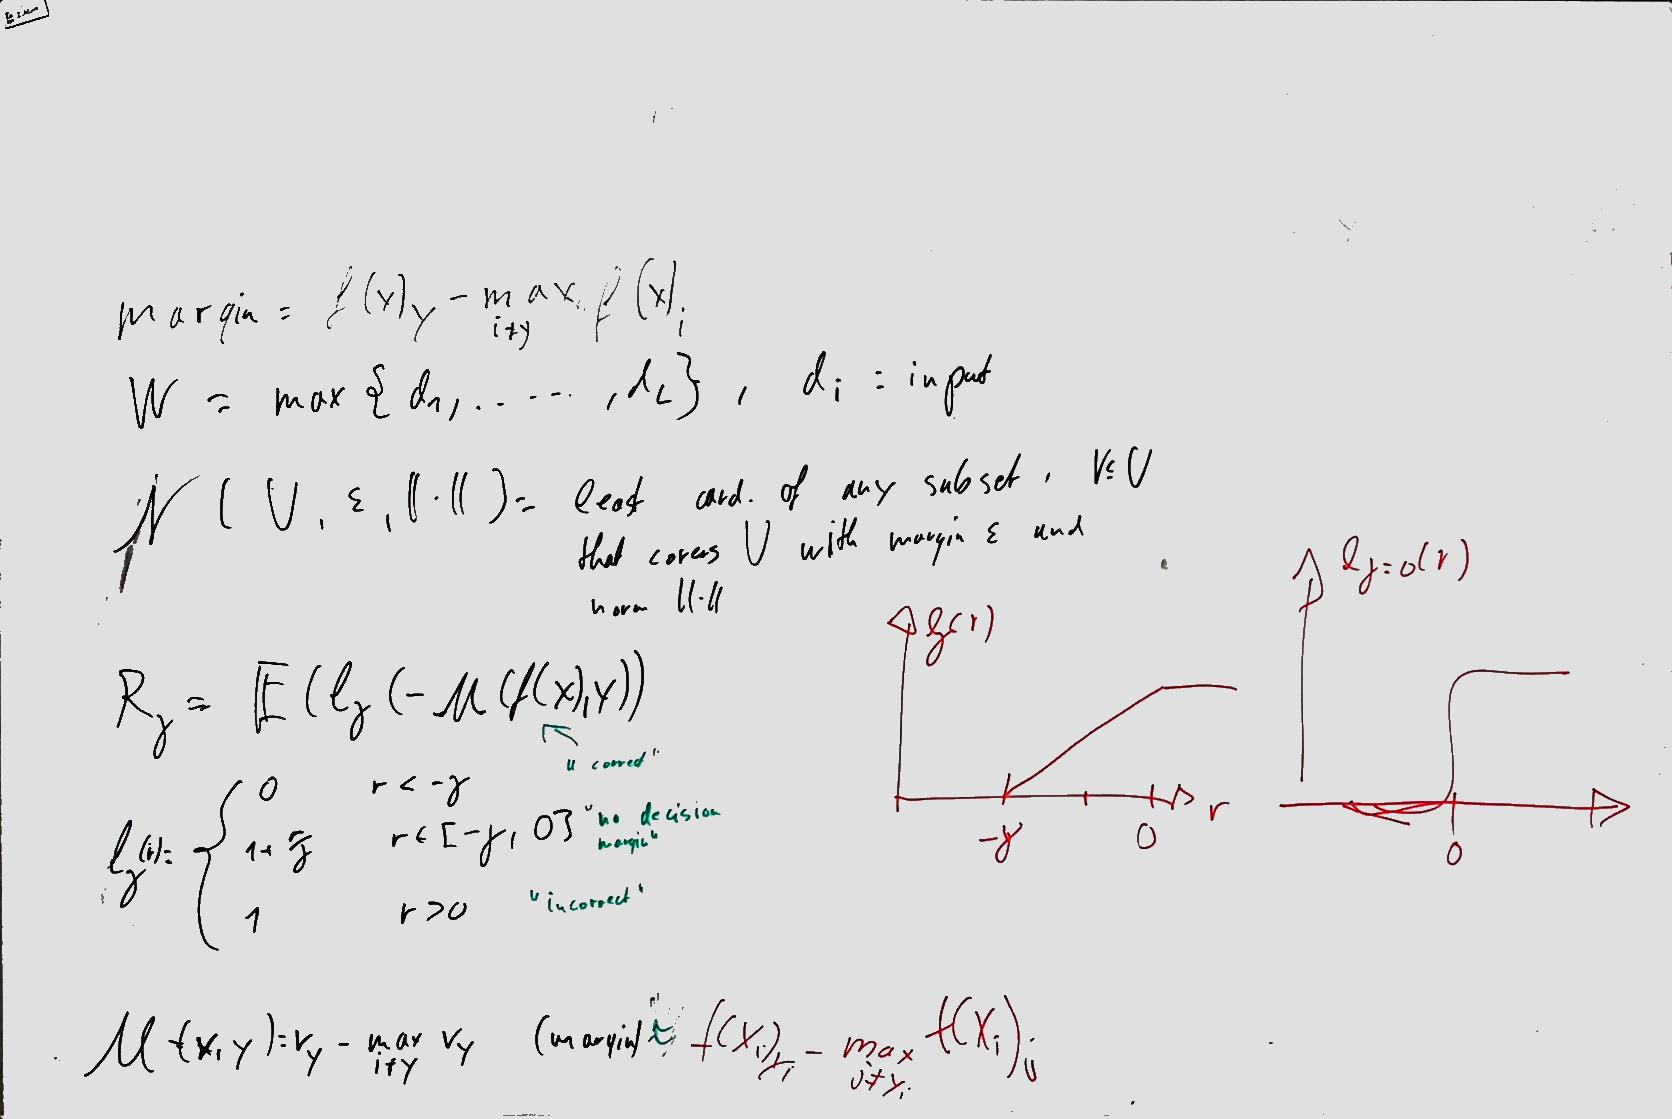
\includegraphics[width=\textwidth]{whiteboard_notes/18.jpg}
\end{figure}

\begin{figure}[htb]
	\centering
	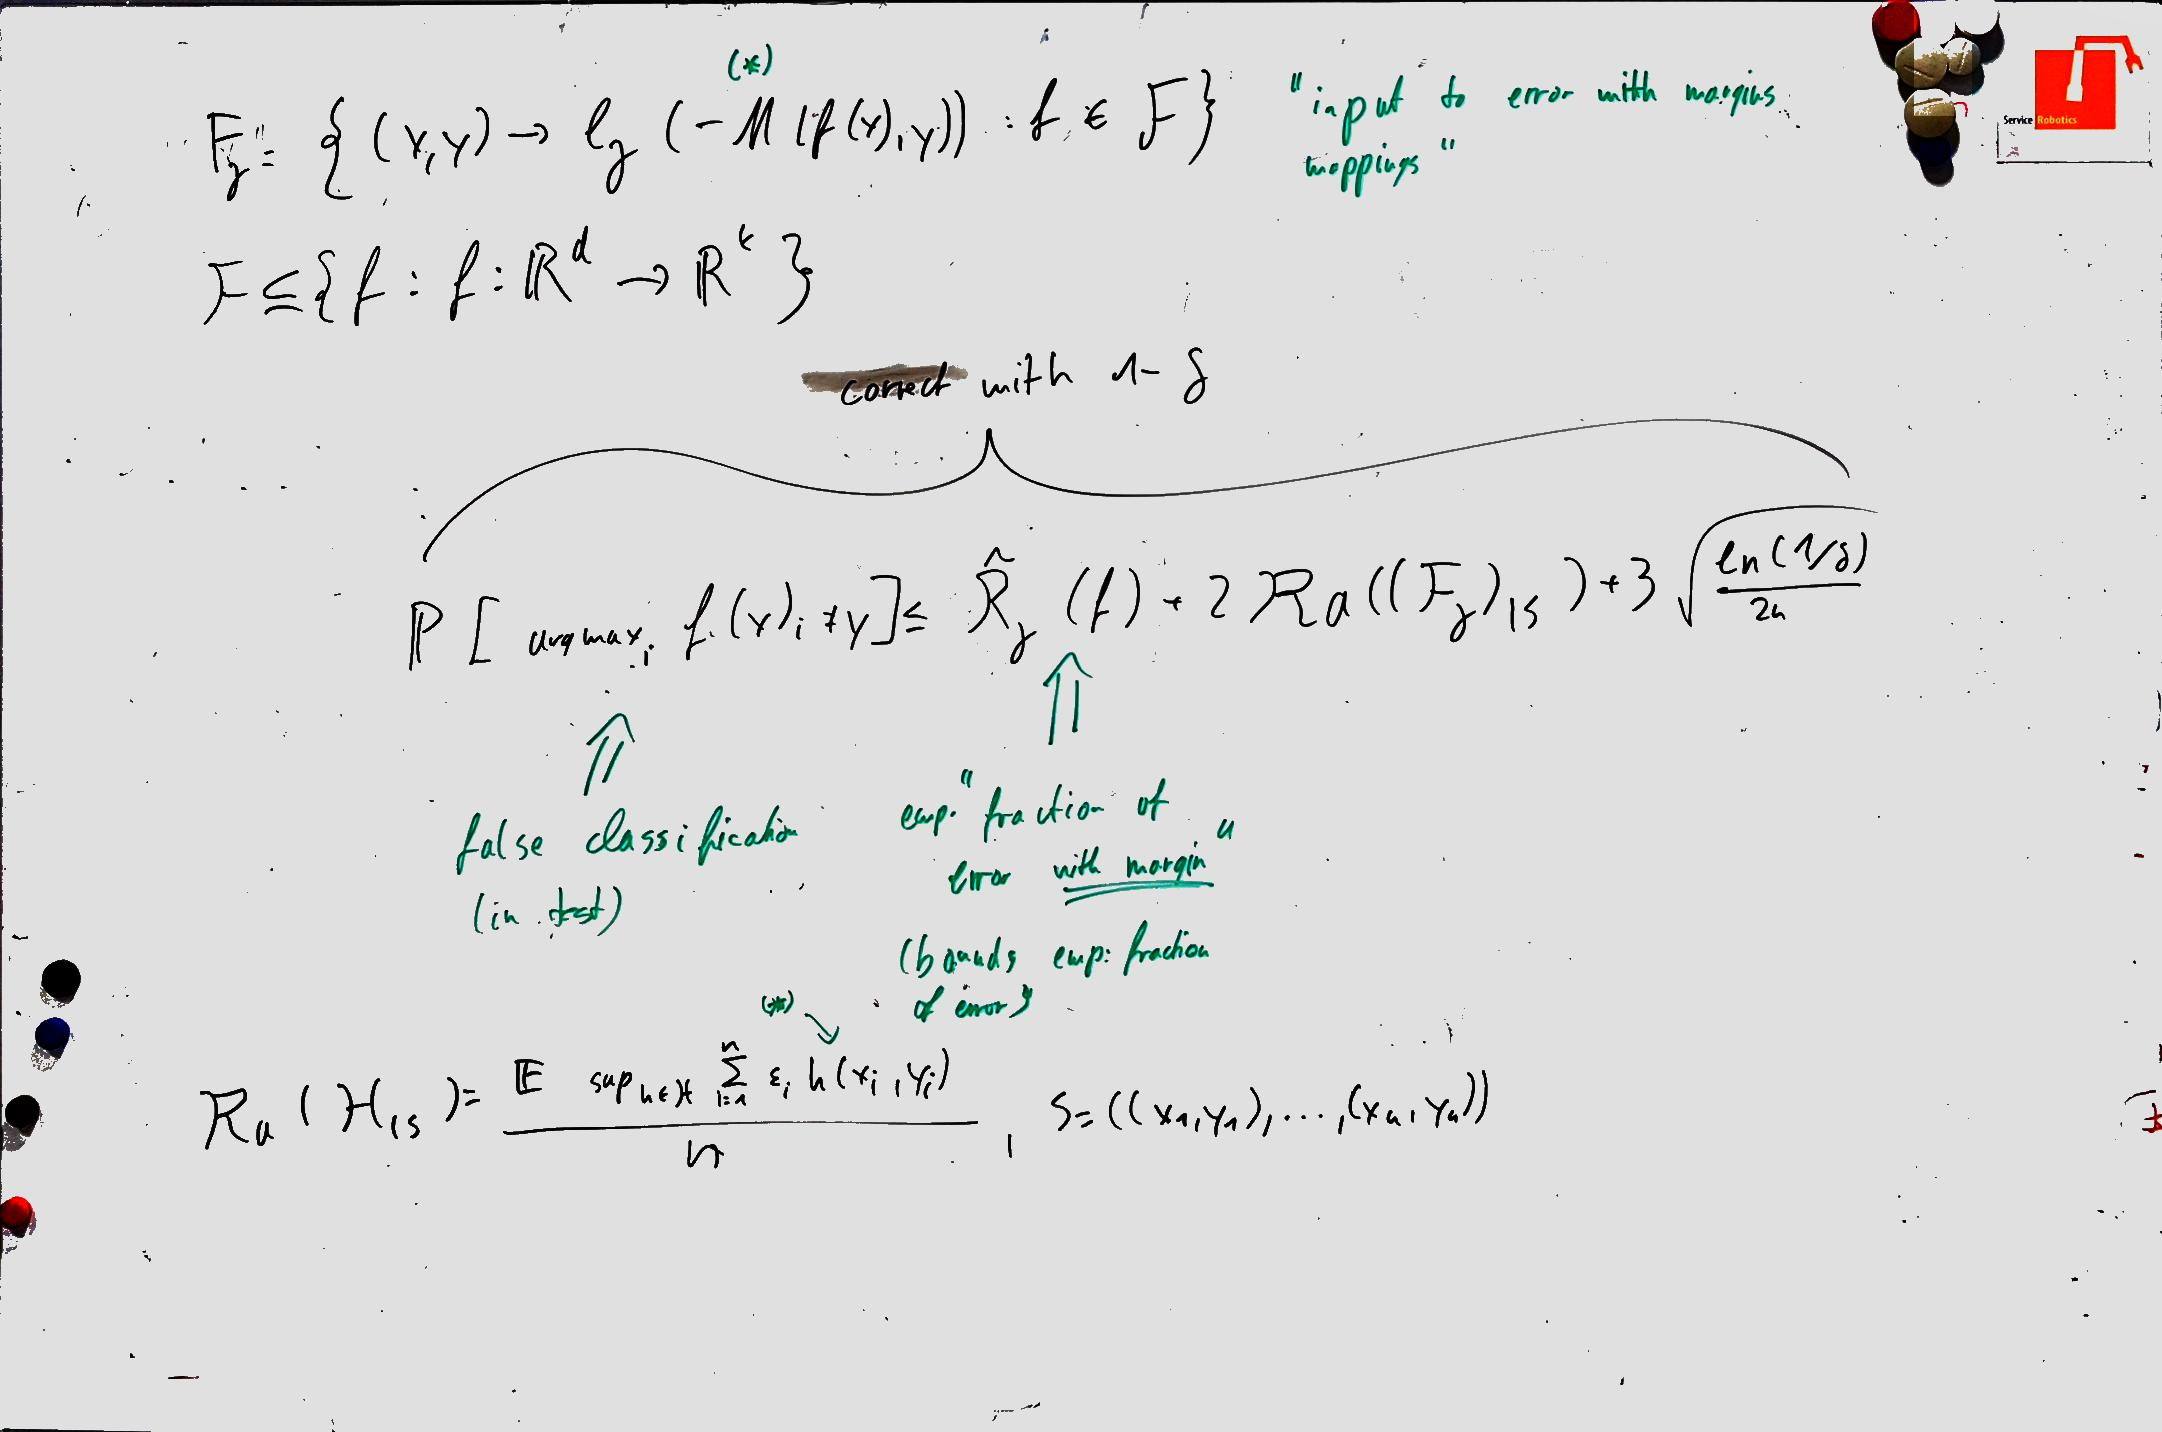
\includegraphics[width=\textwidth]{whiteboard_notes/19.jpg}
\end{figure}

\begin{figure}[htb]
	\centering
	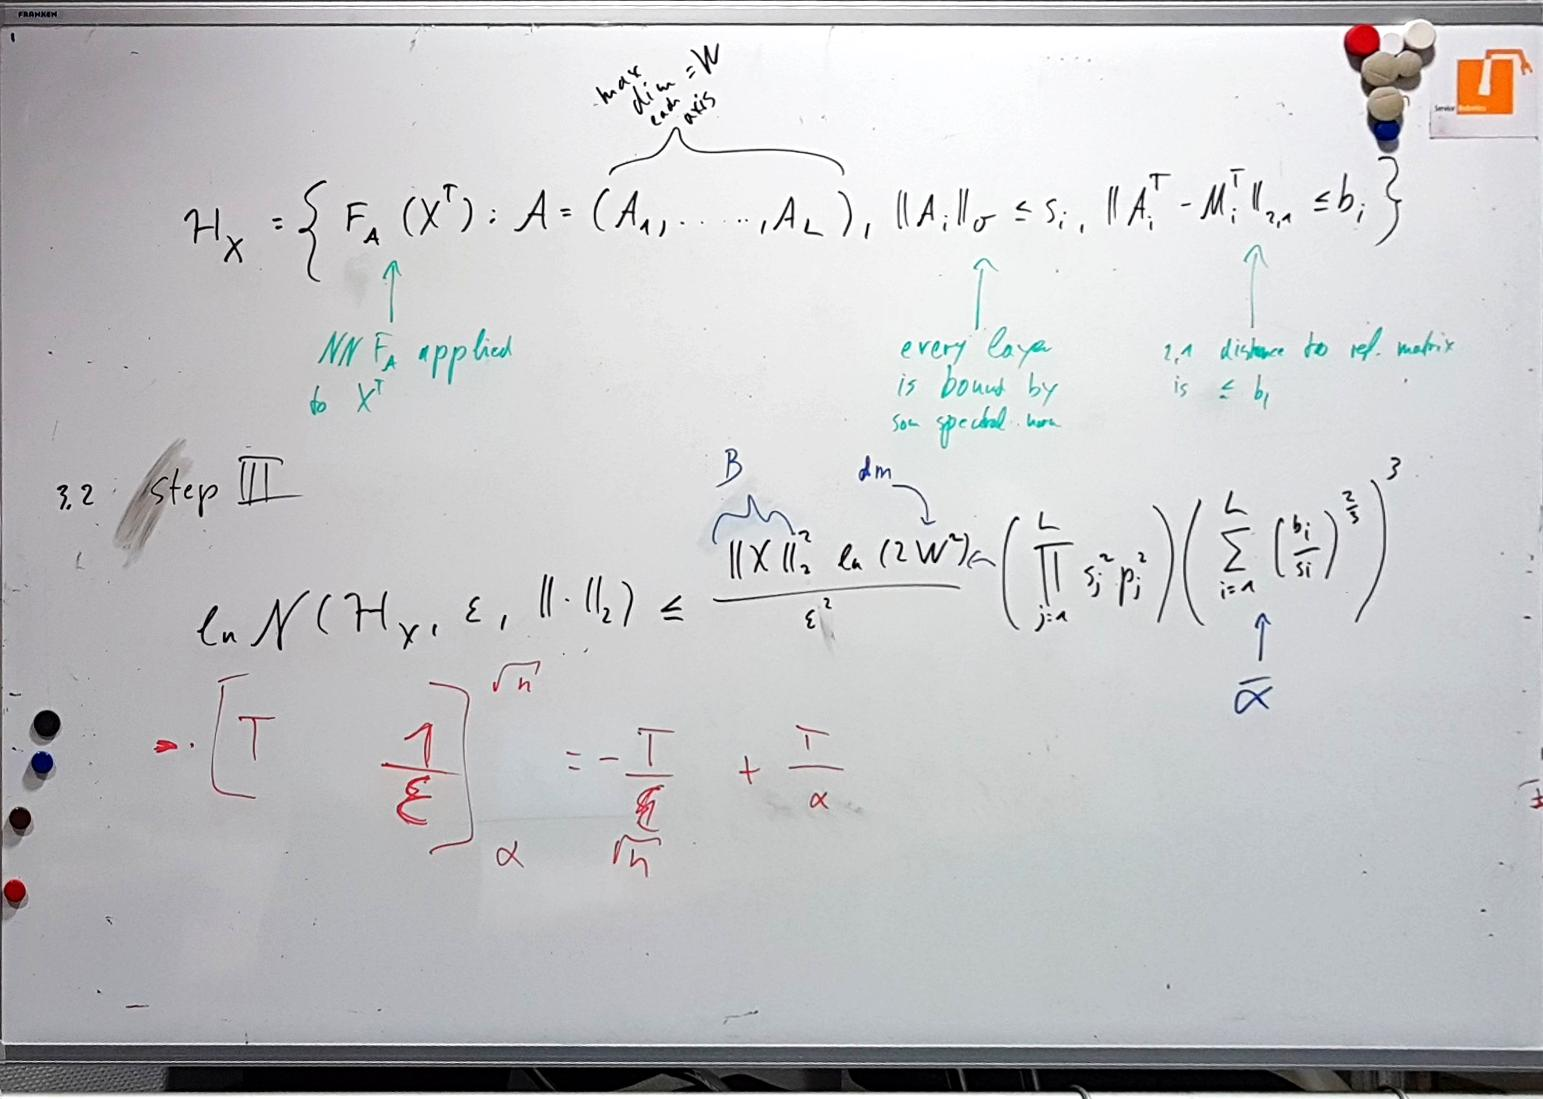
\includegraphics[width=\textwidth]{whiteboard_notes/20.jpg}
\end{figure}

\begin{figure}[htb]
	\centering
	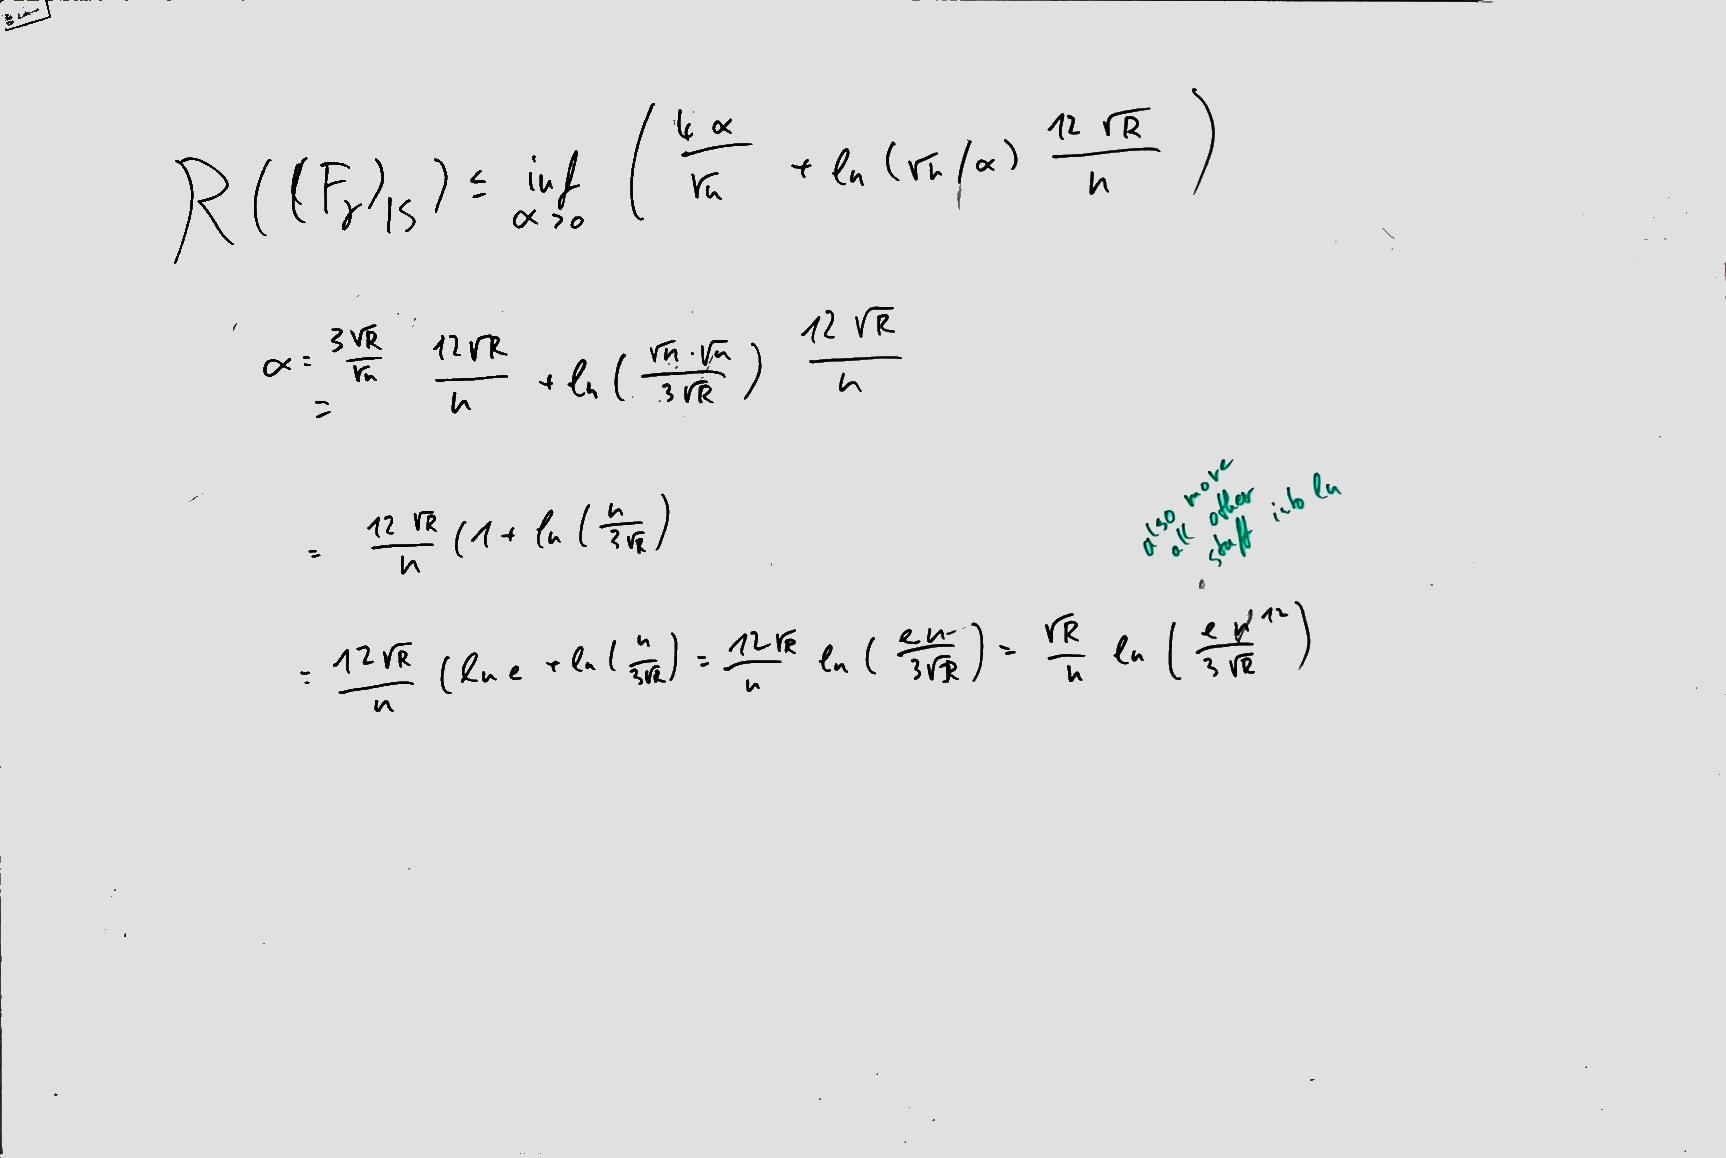
\includegraphics[width=\textwidth]{whiteboard_notes/21.jpg}
\end{figure}


\begin{figure}[htb]
	\centering
	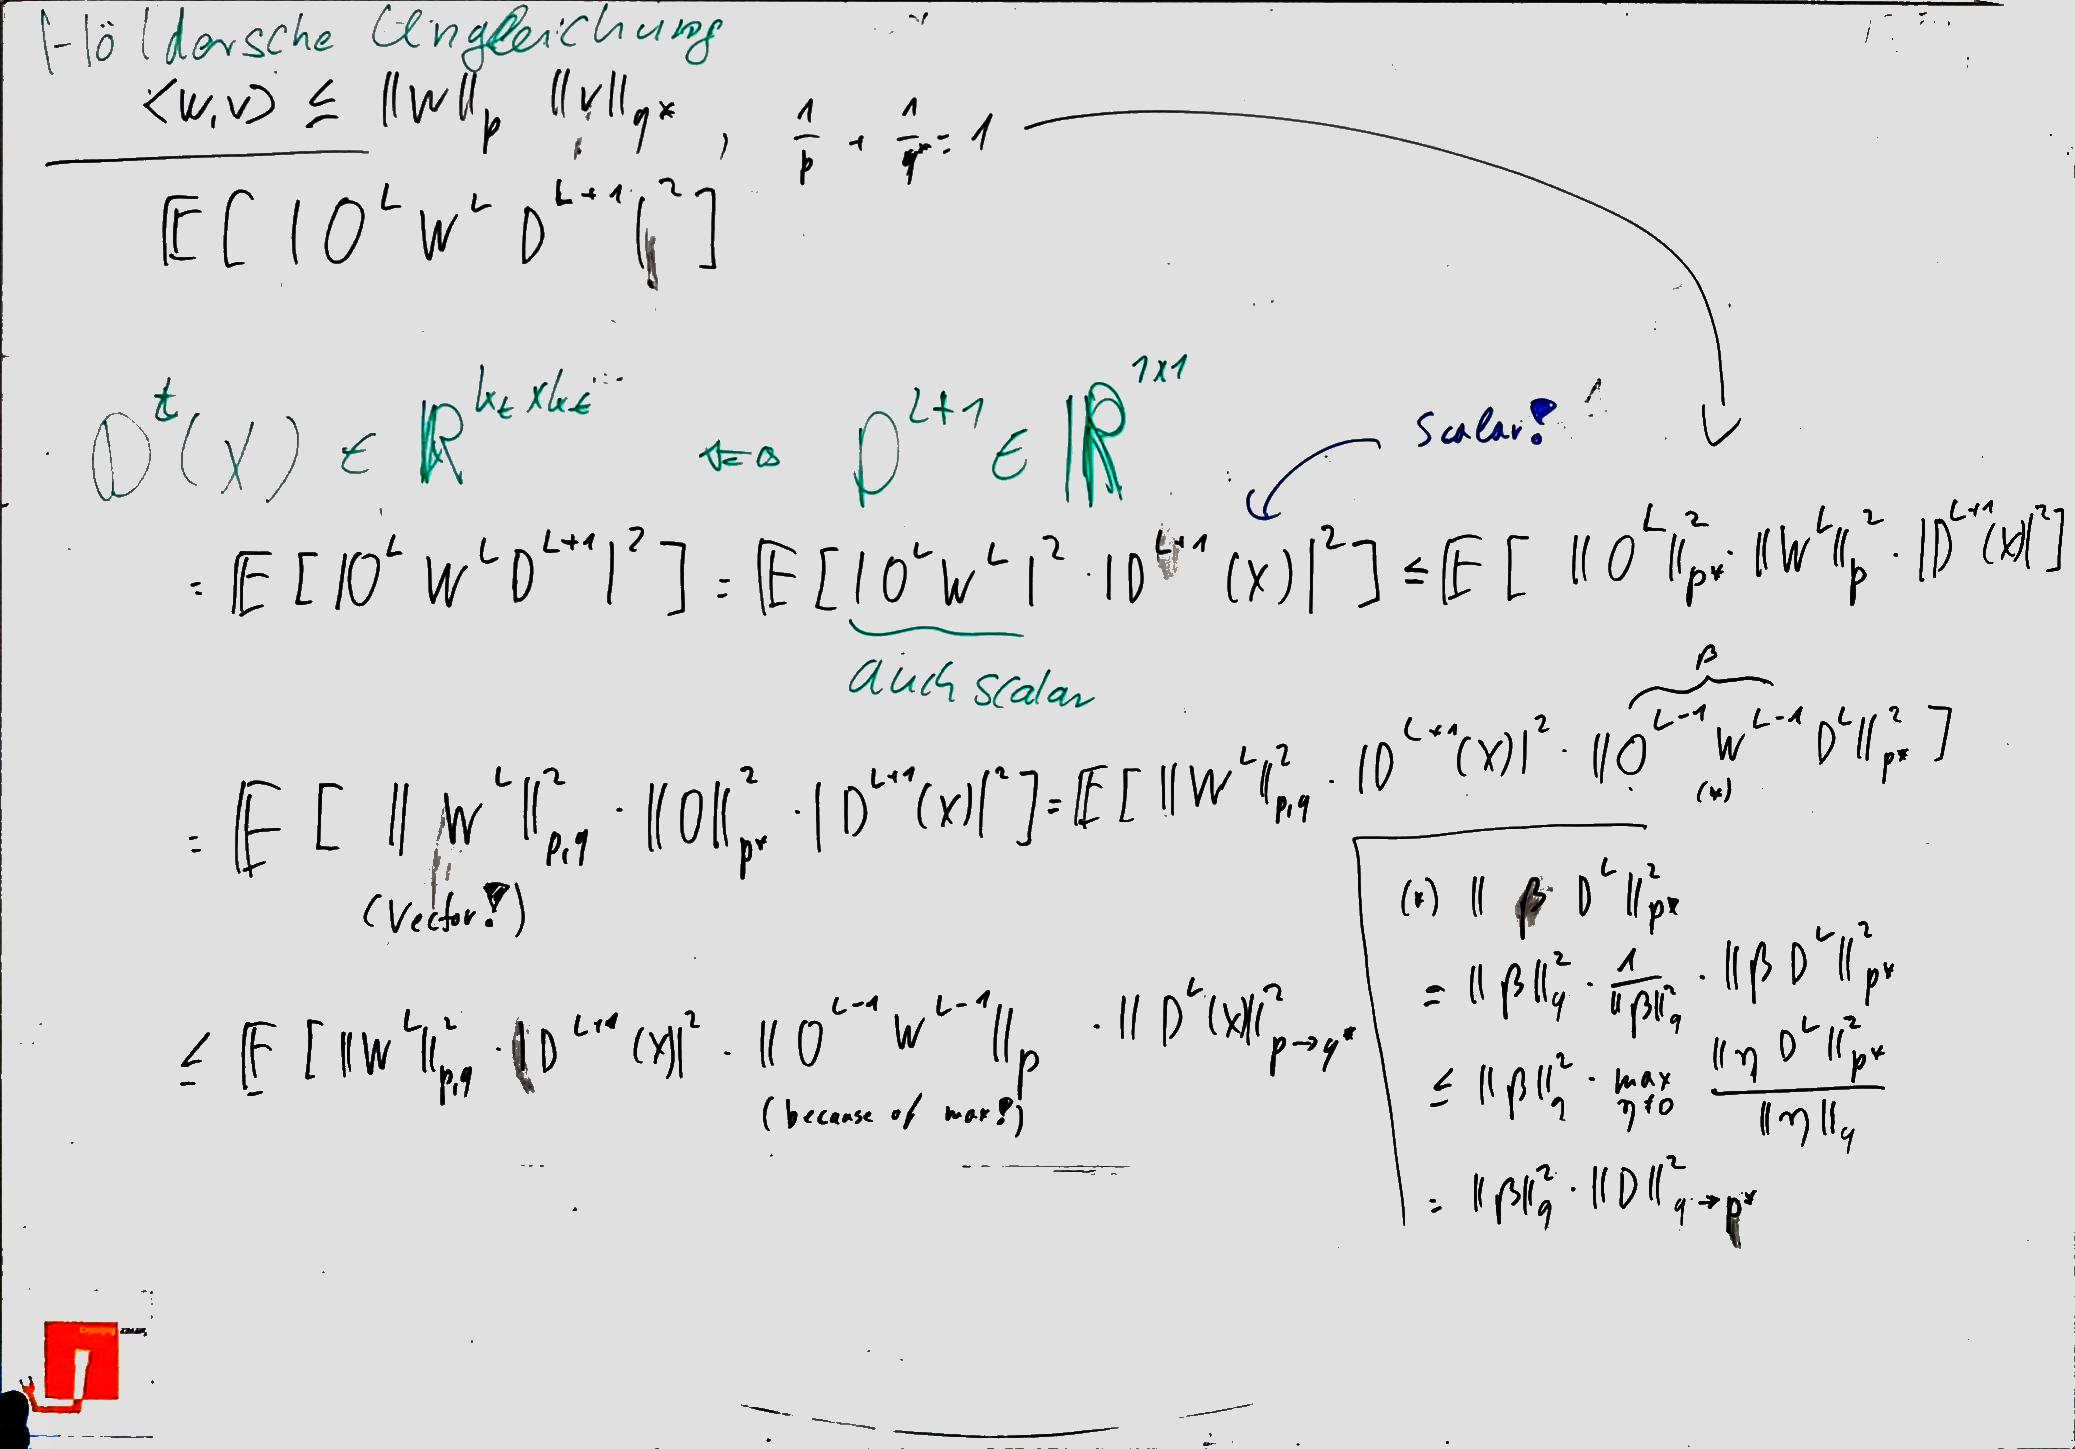
\includegraphics[width=\textwidth]{whiteboard_notes/22.jpg}
\end{figure}

\begin{figure}[htb]
	\centering
	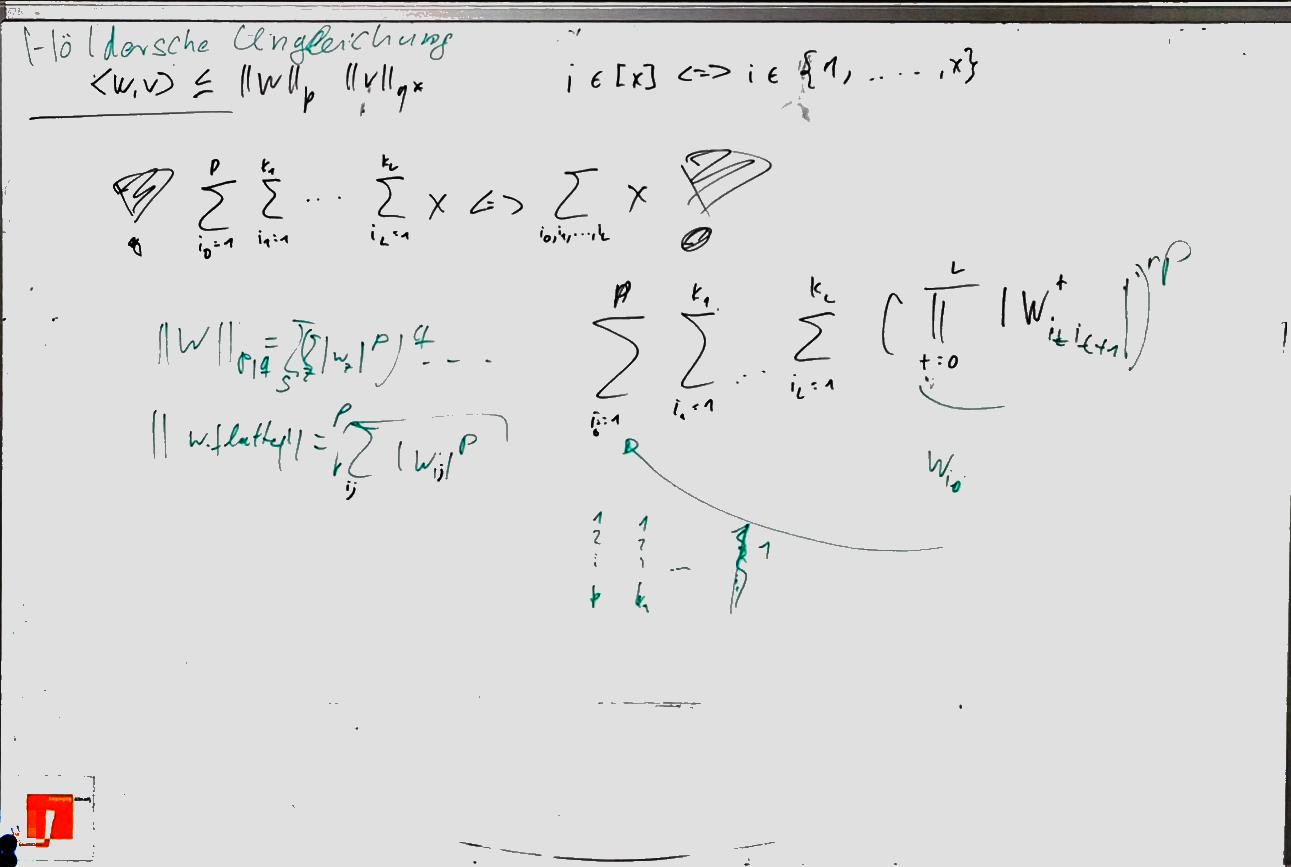
\includegraphics[width=\textwidth]{whiteboard_notes/23.jpg}
\end{figure}

\begin{figure}[htb]
	\centering
	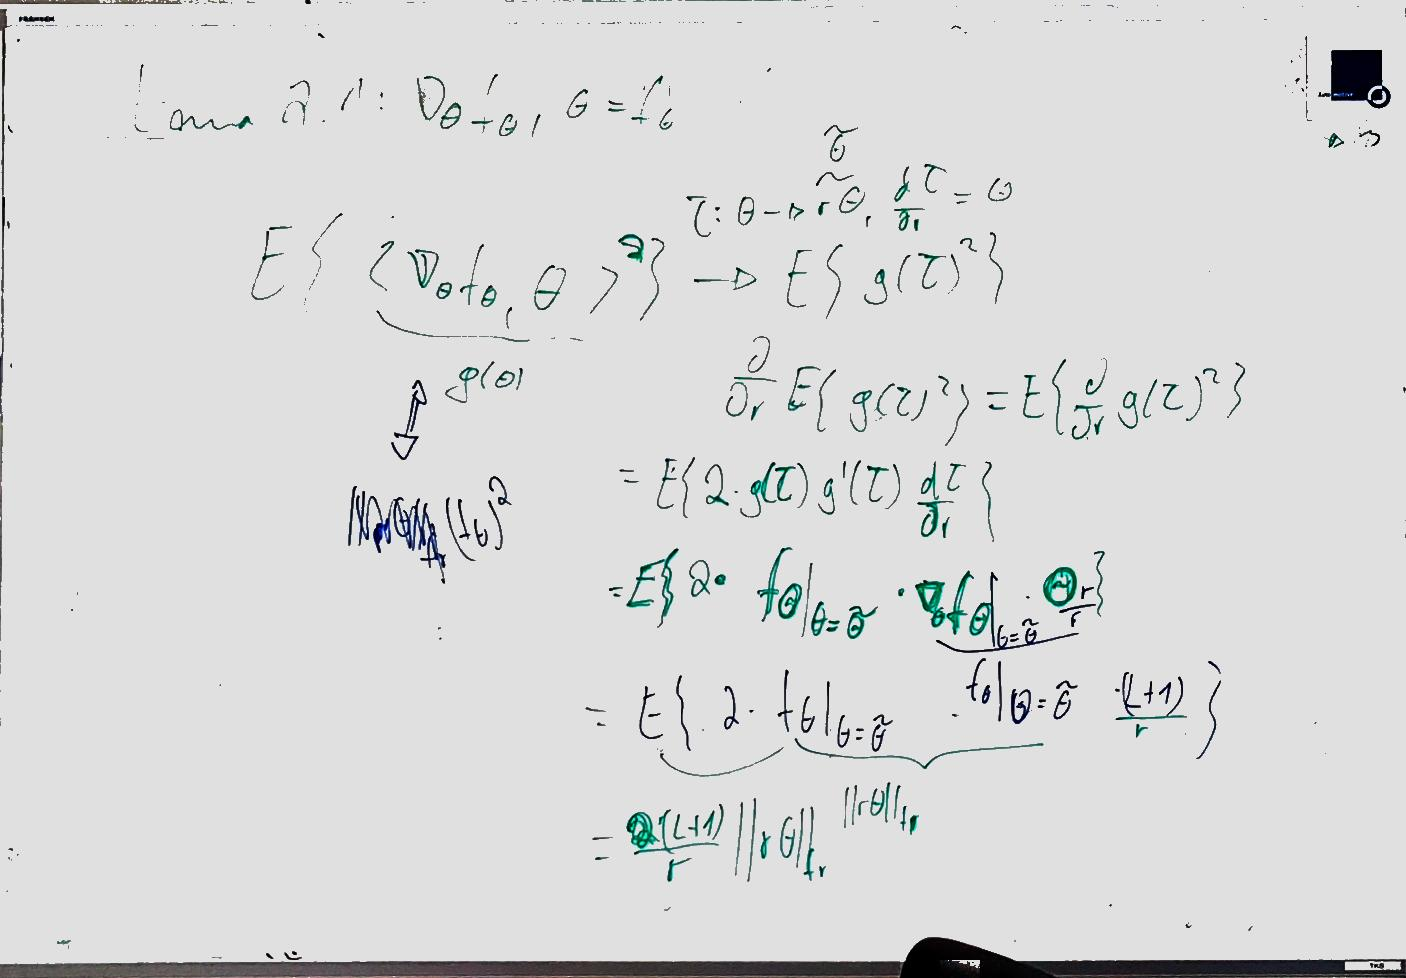
\includegraphics[width=\textwidth]{whiteboard_notes/24.jpg}
\end{figure}

\begin{figure}[htb]
	\centering
	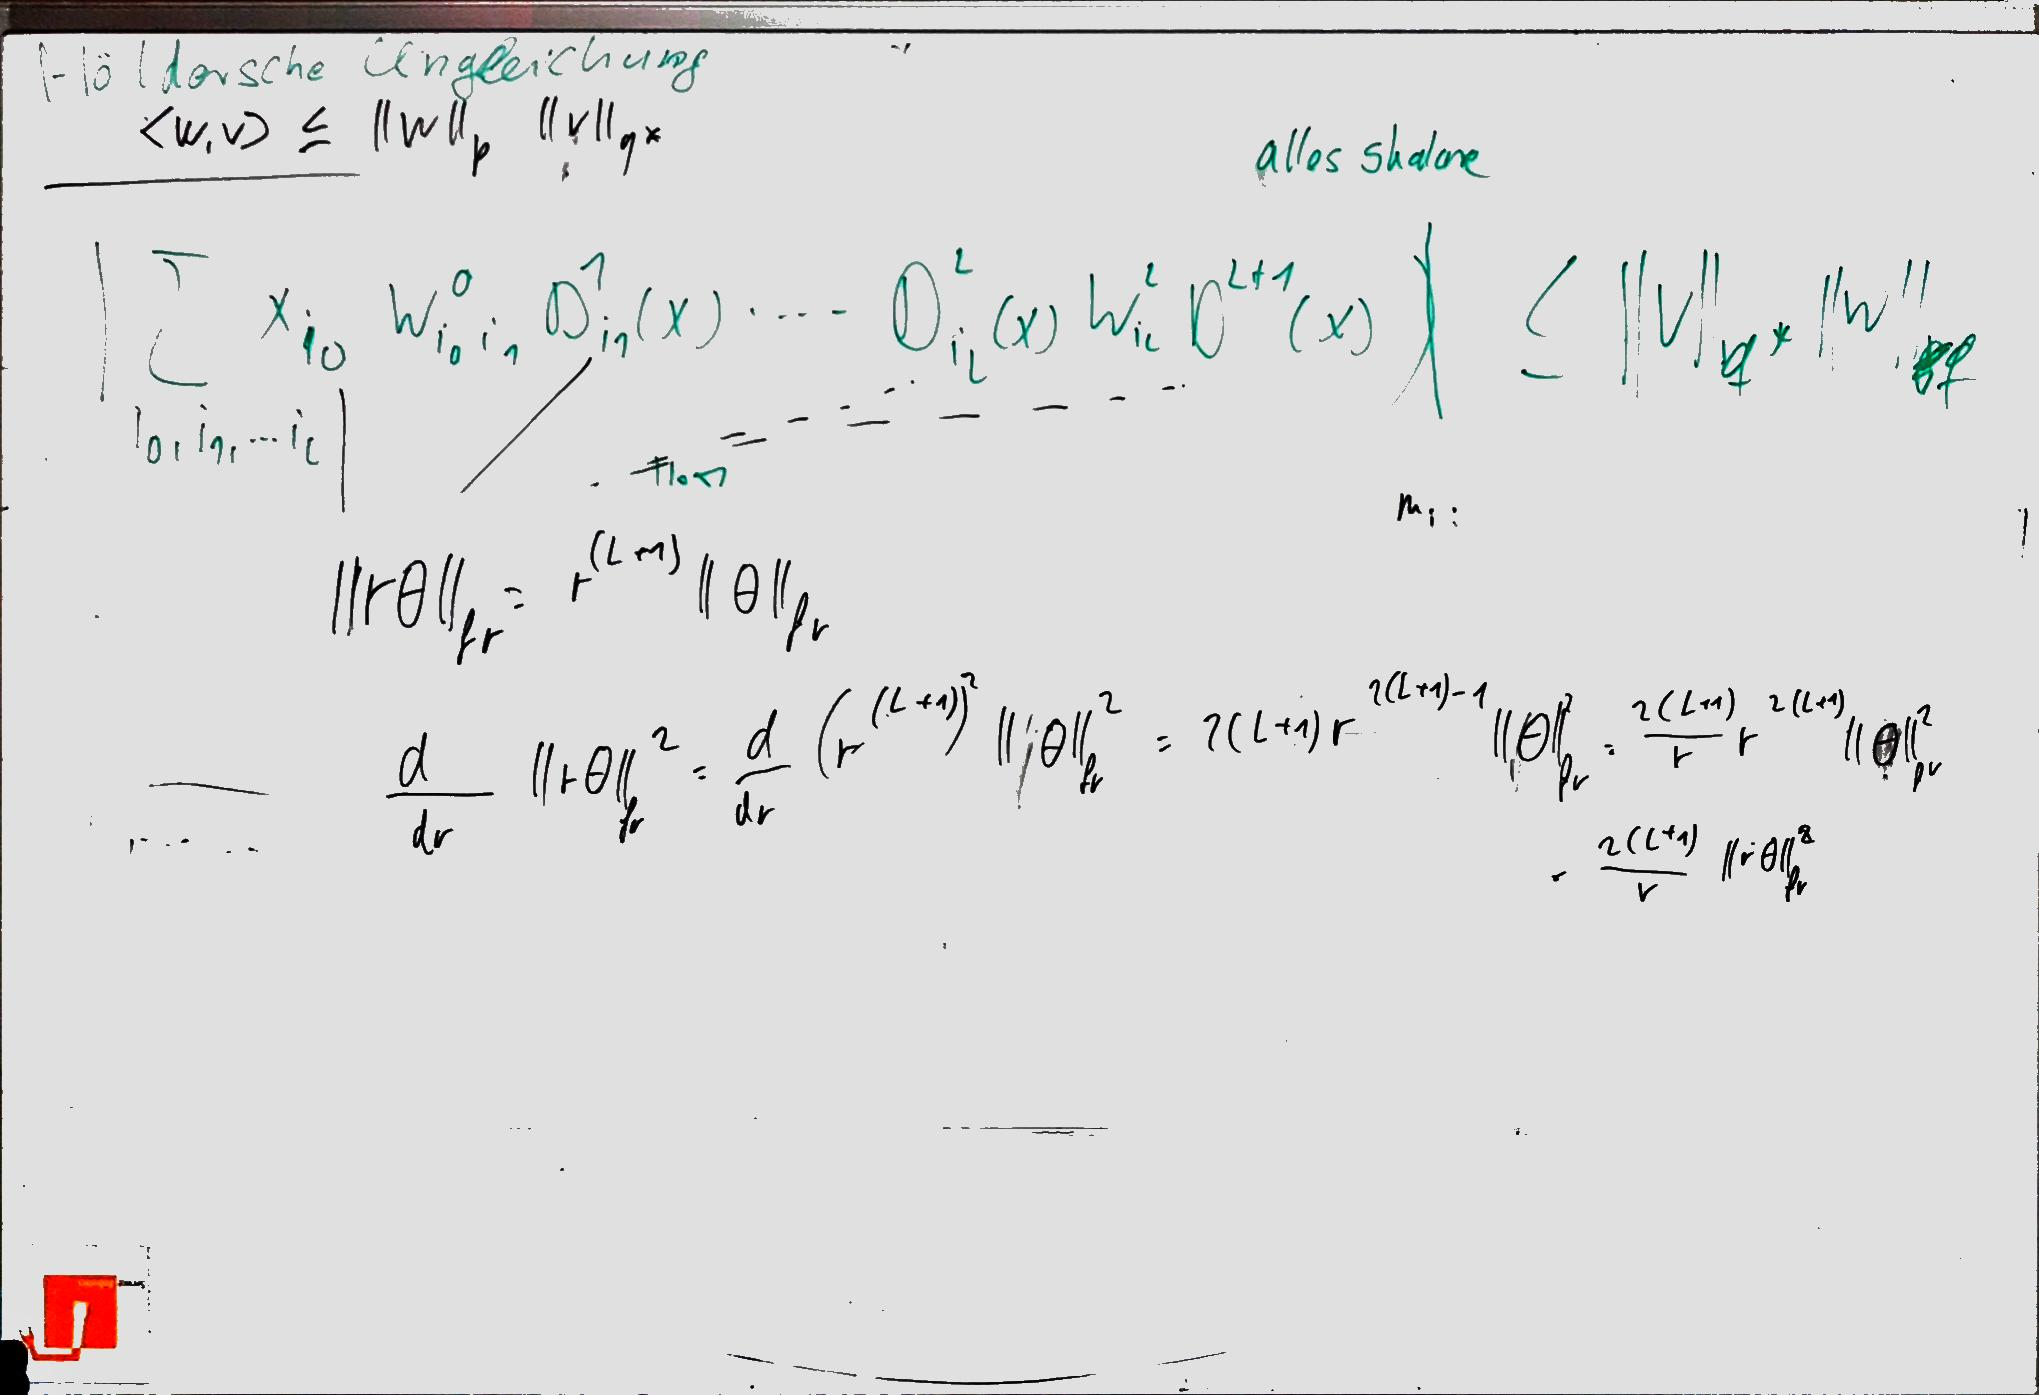
\includegraphics[width=\textwidth]{whiteboard_notes/25.jpg}
\end{figure}

\bibliographystyle{alpha}
\bibliography{sample}

\end{document}